\chapter{Sayısal Tasarım Temelleri}
\label{ch:sayisal-tasarim}
\bolumfoto{gorseller/ekA-galatakulesi.jpg}{Galata Kulesi -- İstanbul}

\section{Giriş}

Mantıksal devre tasarımı (MDT) bilgisayarın ana birimlerden olan veriyolu ve denetiminin tasarımında önemli bir rol oynamaktadır. Bilgisayardaki işlem birimlerinin tasarımı mantıksal devre tasarımı ilkelerine uyularak yapılır. Bölüm~\ref{chap:islemci-tasarimi} ve Bölüm~\ref{chap:boruhatti}'da anlatılan veriyolu tasarımında, birimler ve yazmaçlar birer kutu olarak gösterilmişlerdir. Bu gösterime YAS (Yazmaç Aktarım Seviyesi) denir. YAS'tan bir sonra gelen seviye ise mantıksal tasarım aşamasıdır. Mantıksal tasarım, mantıksal kapıların ve birbirleri ile bağlantılarının ayrıntılı gösterildiği aşamadır. MDT'nin bir alt seviyesi ise elektriksel seviyedir. Bu seviyede tasarımın durumuna göre iyileştirmeler yapacak olan devre elemanlarının tasarımı ve yerleşimi yapılır. Mantık kapıları sayesinde hem karar verme işlemlerinin yapılacağı aşamalar hem de aritmetik işlemler için gereken yapılar kurulabilmektedir. Mantık kapıları tasarlanacak belirli fonksiyonları da yerine getirecek şekilde düzenlenebilmektedir. Bu fonksiyonlardan bazıları çok kullanıldıkları için sabitlenmiş ve çoklayıcı, kodlayıcı, toplayıcı ve yazmaçlar gibi sabit birimler haline getirilmiştir. İkilik düzendeki işlemleri gerçekleştirmek için mantık kapıları kullanılır. Kapılardaki giriş ve çıkış değerleri mantıksal 1 ve 0 sayılarını temsil eden elektriksel değerlerdir. Tasarlanacak birimin verilecek giriş değerlerine göre vereceği sonuçların yazıldığı tabloya doğruluk tablosu denir. Bu bölümde temel mantık kapılarından, doğruluk tabloları ve boole cebrinden, boole fonksiyonlarının sadeleştirilmesinden ve flip-floplardan bahsedilmektedir.


\section{Mantıksal Kapılar ve Doğruluk Tabloları}

\subsection{İkilik Sistem}

Bilgisayarlar ikilik sistemde çalışırlar. İkilik düzendeki sayılar ikiden küçük olan rakamlarla ifade edilir. Her bir basamak ikinin bir kuvvetini temsil eder. Basamakların değerleri sola gidildikçe büyür. İkilik sistemin rakamları olan 1 ve 0 ayrıca mantıktaki doğru ve yanlışı da temsil eder. İkilik sistemdeki bir sayının onluk sisteme çevrilmesinde, onluk tabandaki sayıların çözümlenmesi gibi her rakama karşılık gelen basamağın değeriyle o basamaktaki rakam çarpılır. Çıkan tüm değerler toplanır. Böylece sayının onluk tabandaki değeri elde edilir.

İkilik tabanda yapılan işlemlerden Ek~A'da ayrıntılı olarak bahsedilmektedir.

İkilik sistemde aritmetik işlemler yaparken kullanılan negatif sayılar gösterilirken ikinin tümleyeni yöntemi kullanılır. $R$ tabanında bir $a$ sayının $R$'ye tümleyeni:

\begin{itemize}
    \item $a$ = sayı
    \item $n$ = sayıdaki basamak sayısı
    \item $R$ = sayı tabanı
\end{itemize}

olarak alındığında $R^n - a$ ile bulunur.

\textbf{Örnek:} $(100101)_2$ nin 2'ye tümleyeni:

\[
    2^6 - (100101)_2 = (1000000 - 100101)_2 = (011011)_2
\]


\subsection{Mantık Kapıları ve Doğruluk Tabloları}

Mantık kapıları temel mantıksal fonksiyonları gerçekleştiren transistorler yardımıyla yapılmış olan devrelerdir. Temel mantık fonksiyonları VE, VEYA ve DEĞİL'dir.

\begin{table}[H]
\centering
\begin{minipage}{0.3\textwidth}
\centering
\textbf{VE Kapısı}
\vspace{0.3em}

\begin{tabular}{cc|c}
\toprule
\textbf{A} & \textbf{B} & \textbf{C} \\
\midrule
0 & 0 & 0 \\
0 & 1 & 0 \\
1 & 0 & 0 \\
1 & 1 & 1 \\
\bottomrule
\end{tabular}
\end{minipage}
\hfill
\begin{minipage}{0.3\textwidth}
\centering
\textbf{VEYA Kapısı}
\vspace{0.3em}

\begin{tabular}{cc|c}
\toprule
\textbf{A} & \textbf{B} & \textbf{C} \\
\midrule
0 & 0 & 0 \\
0 & 1 & 1 \\
1 & 0 & 1 \\
1 & 1 & 1 \\
\bottomrule
\end{tabular}
\end{minipage}
\hfill
\begin{minipage}{0.3\textwidth}
\centering
\textbf{DEĞİL Kapısı}
\vspace{0.3em}

\begin{tabular}{c|c}
\toprule
\textbf{A} & \textbf{B} \\
\midrule
0 & 1 \\
1 & 0 \\
\bottomrule
\end{tabular}
\end{minipage}
\end{table}

\begin{figure}[H]
\centering
\begin{tikzpicture}[kapiboy, scale=0.85, transform shape]
  % --- Üst satır: AND, OR, NOT ---
  % AND kapısı
  \node[and gate US, draw, thick, fill=blokgri] (and) at (0,0) {};
  \draw (and.input 1) -- ++(-0.6,0) node[left] {\footnotesize $A$};
  \draw (and.input 2) -- ++(-0.6,0) node[left] {\footnotesize $B$};
  \draw (and.output) -- ++(0.6,0) node[right] {\footnotesize $A \cdot B$};
  \node[below=4pt] at (and.south) {\footnotesize VE (AND)};

  % OR kapısı
  \node[or gate US, draw, thick, fill=blokgri] (or) at (4.5,0) {};
  \draw (or.input 1) -- ++(-0.6,0) node[left] {\footnotesize $A$};
  \draw (or.input 2) -- ++(-0.6,0) node[left] {\footnotesize $B$};
  \draw (or.output) -- ++(0.6,0) node[right] {\footnotesize $A + B$};
  \node[below=4pt] at (or.south) {\footnotesize VEYA (OR)};

  % NOT kapısı
  \node[not gate US, draw, thick, fill=blokgri] (not) at (9,0) {};
  \draw (not.input) -- ++(-0.6,0) node[left] {\footnotesize $A$};
  \draw (not.output) -- ++(0.6,0) node[right] {\footnotesize $\overline{A}$};
  \node[below=4pt] at (not.south) {\footnotesize DEĞİL (NOT)};

  % --- Alt satır: NAND, NOR, XOR ---
  % NAND kapısı
  \node[nand gate US, draw, thick, fill=blokgri] (nand) at (0,-3) {};
  \draw (nand.input 1) -- ++(-0.6,0) node[left] {\footnotesize $A$};
  \draw (nand.input 2) -- ++(-0.6,0) node[left] {\footnotesize $B$};
  \draw (nand.output) -- ++(0.6,0) node[right] {\footnotesize $\overline{A \cdot B}$};
  \node[below=4pt] at (nand.south) {\footnotesize VE DEĞİL (NAND)};

  % NOR kapısı
  \node[nor gate US, draw, thick, fill=blokgri] (nor) at (4.5,-3) {};
  \draw (nor.input 1) -- ++(-0.6,0) node[left] {\footnotesize $A$};
  \draw (nor.input 2) -- ++(-0.6,0) node[left] {\footnotesize $B$};
  \draw (nor.output) -- ++(0.6,0) node[right] {\footnotesize $\overline{A + B}$};
  \node[below=4pt] at (nor.south) {\footnotesize VEYA DEĞİL (NOR)};

  % XOR kapısı
  \node[xor gate US, draw, thick, fill=blokgri] (xor) at (9,-3) {};
  \draw (xor.input 1) -- ++(-0.6,0) node[left] {\footnotesize $A$};
  \draw (xor.input 2) -- ++(-0.6,0) node[left] {\footnotesize $B$};
  \draw (xor.output) -- ++(0.6,0) node[right] {\footnotesize $A \oplus B$};
  \node[below=4pt] at (xor.south) {\footnotesize ÖZEL VEYA (XOR)};
\end{tikzpicture}
\caption{Temel mantık kapıları ve doğruluk tabloları}
\label{fig:B.1}
\end{figure}

Doğruluk tabloları mantık kapılarına girilen verilere göre mantık kapılarının çıkışlarından alınacak değerlerin gösterildiği çizelgelerdir. Doğruluk tablolarında birçok durumun oluşturacağı bir veya birkaç sonuç da gösterilebilmektedir. Eğer gerçekleştirilmek istenen işlem için 5 giriş varsa her girişin 1 ve 0 değerlerini alabileceği göz önüne alınarak, $2^5 = 32$ farklı giriş durumu oluşur.

\begin{table}[H]
\centering
\caption{$v$, $y$, $z$, $m$ ve $n$ giriş, $u$ ve $t$ çıkış değerli $F$ fonksiyonu doğruluk tablosu}
\label{tab:B.1}
\begin{tabular}{ccccc|cc}
\toprule
\textbf{v} & \textbf{y} & \textbf{z} & \textbf{m} & \textbf{n} & \textbf{u} & \textbf{t} \\
\midrule
0 & 0 & 0 & 0 & 0 & 0 & 0 \\
0 & 0 & 0 & 0 & 1 & 0 & 1 \\
0 & 0 & 0 & 1 & 0 & 0 & 1 \\
0 & 0 & 0 & 1 & 1 & 1 & 0 \\
0 & 0 & 1 & 0 & 0 & 0 & 1 \\
0 & 0 & 1 & 0 & 1 & 1 & 0 \\
0 & 0 & 1 & 1 & 0 & 1 & 0 \\
0 & 0 & 1 & 1 & 1 & 1 & 1 \\
0 & 1 & 0 & 0 & 0 & 0 & 1 \\
0 & 1 & 0 & 0 & 1 & 1 & 0 \\
0 & 1 & 0 & 1 & 0 & 1 & 0 \\
0 & 1 & 0 & 1 & 1 & 1 & 1 \\
0 & 1 & 1 & 0 & 0 & 1 & 0 \\
0 & 1 & 1 & 0 & 1 & 1 & 1 \\
0 & 1 & 1 & 1 & 0 & 1 & 1 \\
0 & 1 & 1 & 1 & 1 & 0 & 0 \\
1 & 0 & 0 & 0 & 0 & 0 & 1 \\
1 & 0 & 0 & 0 & 1 & 1 & 0 \\
1 & 0 & 0 & 1 & 0 & 1 & 0 \\
1 & 0 & 0 & 1 & 1 & 1 & 1 \\
1 & 0 & 1 & 0 & 0 & 1 & 0 \\
1 & 0 & 1 & 0 & 1 & 1 & 1 \\
1 & 0 & 1 & 1 & 0 & 1 & 1 \\
1 & 0 & 1 & 1 & 1 & 0 & 0 \\
1 & 1 & 0 & 0 & 0 & 1 & 0 \\
1 & 1 & 0 & 0 & 1 & 1 & 1 \\
1 & 1 & 0 & 1 & 0 & 1 & 1 \\
1 & 1 & 0 & 1 & 1 & 0 & 0 \\
1 & 1 & 1 & 0 & 0 & 1 & 1 \\
1 & 1 & 1 & 0 & 1 & 0 & 0 \\
1 & 1 & 1 & 1 & 0 & 0 & 0 \\
1 & 1 & 1 & 1 & 1 & 0 & 1 \\
\bottomrule
\end{tabular}
\end{table}


\section{Boole Cebri}

Boole cebri 1854 yılında George Boole tarafından geliştirilmiştir. Boole cebri mantıksal işlemlerin formülleştirilmesinde kullanılır. Matematikte tanımlanan işlemler belirli özellikleri sağladıkları zaman cebir olarak kabul edilirler. Bu özelliklerin neler olacağı konusunda farklı önermeler vardır. Boole cebri için kabul edilen Huntington önermeleridir. Boole cebrinde temel işlemler olan VE ve VEYA sırasıyla ``$\cdot$'' ve ``$+$'' işaretleriyle gösterilirler. Bu işlemler matematikteki çarpma ve toplama işlemlerine benzer özellikler gösterir.

Boole cebrinin temel özellikleri şunlardır:

\begin{itemize}
    \item \textbf{Kapalılık:} $1 + 1 = 1$ (1 VEYA 1 eşittir 1)
    \item \textbf{Birim eleman:} ``$\cdot$'' için 1: $x \cdot 1 = x$; ``$+$'' için 0: $x + 0 = x$
    \item \textbf{Değişme:} $x + y = y + x$ ve $x \cdot y = y \cdot x$
    \item \textbf{Dağılma:} $x \cdot (y + z) = (x \cdot y) + (x \cdot z)$ ve $x + (y \cdot z) = (x + y) \cdot (x + z)$
    \item \textbf{Ters:} $x + \overline{x} = 1$ ve $x \cdot \overline{x} = 0$
\end{itemize}

\begin{table}[H]
\centering
\caption{``$\cdot$'', ``$+$'' ve ``DEĞİL'' doğruluk tabloları}
\label{tab:B.2}
\begin{minipage}{0.3\textwidth}
\centering
\textbf{VE ($\cdot$)}
\vspace{0.3em}

\begin{tabular}{cc|c}
\toprule
$x$ & $y$ & $x \cdot y$ \\
\midrule
0 & 0 & 0 \\
0 & 1 & 0 \\
1 & 0 & 0 \\
1 & 1 & 1 \\
\bottomrule
\end{tabular}
\end{minipage}
\hfill
\begin{minipage}{0.3\textwidth}
\centering
\textbf{VEYA ($+$)}
\vspace{0.3em}

\begin{tabular}{cc|c}
\toprule
$x$ & $y$ & $x + y$ \\
\midrule
0 & 0 & 0 \\
0 & 1 & 1 \\
1 & 0 & 1 \\
1 & 1 & 1 \\
\bottomrule
\end{tabular}
\end{minipage}
\hfill
\begin{minipage}{0.3\textwidth}
\centering
\textbf{DEĞİL}
\vspace{0.3em}

\begin{tabular}{c|c}
\toprule
$x$ & $\overline{x}$ \\
\midrule
0 & 1 \\
1 & 0 \\
\bottomrule
\end{tabular}
\end{minipage}
\end{table}

\begin{table}[H]
\centering
\caption{$F_1 = x y \overline{z}$, $F_2 = x + \overline{y} + \overline{z}$, $F_3 = \overline{x}(y + z)$ fonksiyonlarının doğruluk tablosu}
\label{tab:B.3}
\begin{tabular}{ccc|ccc}
\toprule
$x$ & $y$ & $z$ & $F_1 = x y \overline{z}$ & $F_2 = x + \overline{y} + \overline{z}$ & $F_3 = \overline{x}(y + z)$ \\
\midrule
0 & 0 & 0 & 0 & 1 & 0 \\
0 & 0 & 1 & 0 & 1 & 0 \\
0 & 1 & 0 & 0 & 1 & 1 \\
0 & 1 & 1 & 0 & 0 & 1 \\
1 & 0 & 0 & 0 & 1 & 0 \\
1 & 0 & 1 & 0 & 1 & 0 \\
1 & 1 & 0 & 1 & 1 & 0 \\
1 & 1 & 1 & 0 & 1 & 0 \\
\bottomrule
\end{tabular}
\end{table}

\begin{figure}[H]
\centering
\begin{tikzpicture}[kapiboy, scale=0.85, transform shape]
  % NOT kapısı (z'nin tersi)
  \node[not gate US, draw, thick, fill=blokgri] (notz) at (1.5, -1) {};
  % AND kapısı (3 girişli)
  \node[and gate US, draw, thick, fill=blokgri, inputs={nnn}] (and1) at (4.5, 0) {};

  % Girişler
  \draw (and1.input 1) -- ++(-2.2,0) node[left] {\footnotesize $x$};
  \draw (and1.input 2) -- ++(-2.2,0) node[left] {\footnotesize $y$};
  \draw (notz.input) -- ++(-0.6,0) node[left] {\footnotesize $z$};
  \draw (notz.output) -- (and1.input 3 -| notz.output) -- (and1.input 3);

  % Çıkış
  \draw (and1.output) -- ++(0.8,0) node[right] {\footnotesize $F_1 = x \cdot y \cdot \overline{z}$};
\end{tikzpicture}
\caption{$F_1$ fonksiyonunun mantık kapıları ile gösterimi}
\label{fig:B.2}
\end{figure}

\begin{figure}[H]
\centering
\begin{tikzpicture}[kapiboy, scale=0.85, transform shape]
  % NOT kapıları
  \node[not gate US, draw, thick, fill=blokgri] (noty) at (1.5, 0) {};
  \node[not gate US, draw, thick, fill=blokgri] (notz) at (1.5, -1.2) {};
  % OR kapısı (3 girişli)
  \node[or gate US, draw, thick, fill=blokgri, inputs={nnn}] (or1) at (4.5, 0) {};

  % Girişler
  \draw (or1.input 1) -- ++(-2.2,0) node[left] {\footnotesize $x$};
  \draw (noty.input) -- ++(-0.6,0) node[left] {\footnotesize $y$};
  \draw (noty.output) -- (or1.input 2 -| noty.output) -- (or1.input 2);
  \draw (notz.input) -- ++(-0.6,0) node[left] {\footnotesize $z$};
  \draw (notz.output) -- (or1.input 3 -| notz.output) -- (or1.input 3);

  % Çıkış
  \draw (or1.output) -- ++(0.8,0) node[right] {\footnotesize $F_2 = x + \overline{y} + \overline{z}$};
\end{tikzpicture}
\caption{$F_2$ fonksiyonunun mantık kapıları ile gösterimi}
\label{fig:B.3}
\end{figure}

\begin{figure}[H]
\centering
\begin{tikzpicture}[kapiboy, scale=0.85, transform shape]
  % NOT kapısı (x'in tersi)
  \node[not gate US, draw, thick, fill=blokgri] (notx) at (1.5, 0.6) {};
  % OR kapısı (y + z)
  \node[or gate US, draw, thick, fill=blokgri] (or1) at (2.5, -0.8) {};
  % AND kapısı
  \node[and gate US, draw, thick, fill=blokgri] (and1) at (5.5, 0) {};

  % Girişler
  \draw (notx.input) -- ++(-0.6,0) node[left] {\footnotesize $x$};
  \draw (or1.input 1) -- ++(-1.6,0) node[left] {\footnotesize $y$};
  \draw (or1.input 2) -- ++(-1.6,0) node[left] {\footnotesize $z$};

  % Bağlantılar
  \draw (notx.output) -- (and1.input 1 -| notx.output) -- (and1.input 1);
  \draw (or1.output) -- (and1.input 2 -| or1.output) -- (and1.input 2);

  % Çıkış
  \draw (and1.output) -- ++(0.8,0) node[right] {\footnotesize $F_3 = \overline{x}(y + z)$};
\end{tikzpicture}
\caption{$F_3$ fonksiyonunun mantık kapıları ile gösterimi}
\label{fig:B.4}
\end{figure}


\subsection{Mini Terimler ve Maksi Terimler}

Fonksiyonların bir başka gösterim şekli de maksi terimler ve mini terimlerdir. Mini terimler değişkenlerin değerlerinin VE işlemleri ile ifade edilmesi, maksi terimleri ise VEYA işlemleri ile ifade edilmesidir.

\begin{table}[H]
\centering
\caption{Mini ve maksi terimlerin gösterimi}
\label{tab:B.4}
\begin{tabular}{ccc|cc|cc}
\toprule
$x$ & $y$ & $z$ & \textbf{Mini Terim} & \textbf{Sembol} & \textbf{Maksi Terim} & \textbf{Sembol} \\
\midrule
0 & 0 & 0 & $\overline{x}\,\overline{y}\,\overline{z}$ & $m_0$ & $x+y+z$ & $M_0$ \\
0 & 0 & 1 & $\overline{x}\,\overline{y}\,z$ & $m_1$ & $x+y+\overline{z}$ & $M_1$ \\
0 & 1 & 0 & $\overline{x}\,y\,\overline{z}$ & $m_2$ & $x+\overline{y}+z$ & $M_2$ \\
0 & 1 & 1 & $\overline{x}\,y\,z$ & $m_3$ & $x+\overline{y}+\overline{z}$ & $M_3$ \\
1 & 0 & 0 & $x\,\overline{y}\,\overline{z}$ & $m_4$ & $\overline{x}+y+z$ & $M_4$ \\
1 & 0 & 1 & $x\,\overline{y}\,z$ & $m_5$ & $\overline{x}+y+\overline{z}$ & $M_5$ \\
1 & 1 & 0 & $x\,y\,\overline{z}$ & $m_6$ & $\overline{x}+\overline{y}+z$ & $M_6$ \\
1 & 1 & 1 & $x\,y\,z$ & $m_7$ & $\overline{x}+\overline{y}+\overline{z}$ & $M_7$ \\
\bottomrule
\end{tabular}
\end{table}

Fonksiyonların mini terimler ve maksi terimlerle gösterilebilmeleri için belirli bir formda yazılmaları gerekir. Mini terimler toplamı $\Sigma$ gösterimi ile, maksi terimler çarpımı ise $\Pi$ gösterimi ile ifade edilir.

\begin{ornek}[B.1]
$F_1$ ve $F_2$ fonksiyonlarını miniterimler ve $\Sigma$ işaretiyle gösterin.

\textbf{Çözüm B.1}

Doğruluk tablosundan $F_1$ ve $F_2$ fonksiyonlarının 1 değerini aldığı satırlar belirlenir:

\[
    F_1 = m_3 + m_4 + m_6 = \overline{x}\,y\,z + x\,\overline{y}\,\overline{z} + x\,y\,\overline{z} = \Sigma(3,4,6)
\]
\[
    F_2 = m_0 + m_3 + m_7 = \overline{x}\,\overline{y}\,\overline{z} + \overline{x}\,y\,z + x\,y\,z = \Sigma(0,3,7)
\]
\end{ornek}

\begin{table}[H]
\centering
\caption{Standart Mantık İşlemleri}
\label{tab:B.5}
\begin{tabular}{clll}
\toprule
\textbf{Fonksiyon} & \textbf{Sembol} & \textbf{Ad} & \textbf{Açıklama} \\
\midrule
$0$ & -- & Boş & Her zaman 0 \\
$x \cdot y$ & VE & VE & Her ikisi de 1 ise 1 \\
$x \cdot \overline{y}$ & -- & Engelleme & $x=1$ ve $y=0$ ise 1 \\
$x$ & -- & Aktarım & $x$ değeri \\
$\overline{x} \cdot y$ & -- & Engelleme & $x=0$ ve $y=1$ ise 1 \\
$y$ & -- & Aktarım & $y$ değeri \\
$x\overline{y} + \overline{x}y$ & $\oplus$ & Özel VEYA & Farklı ise 1 \\
$x + y$ & VEYA & VEYA & En az biri 1 ise 1 \\
$\overline{(x + y)}$ & VEYA DEĞİL & VEYA DEĞİL & Her ikisi de 0 ise 1 \\
$x y + \overline{x}\,\overline{y}$ & $\odot$ & Eşdeğerlik & Aynı ise 1 \\
$\overline{y}$ & -- & Tümleyen & $y$'nin tersi \\
$x + \overline{y}$ & -- & İçerme & $x=1$ veya $y=0$ ise 1 \\
$\overline{x}$ & -- & Tümleyen & $x$'in tersi \\
$\overline{x} + y$ & -- & İçerme & $x=0$ veya $y=1$ ise 1 \\
$\overline{(x \cdot y)}$ & VE DEĞİL & VE DEĞİL & En az biri 0 ise 1 \\
$1$ & -- & Birim Eleman & Her zaman 1 \\
\bottomrule
\end{tabular}
\end{table}

\begin{table}[H]
\centering
\caption{ÖZEL VEYA, VE DEĞİL, VEYA DEĞİL ve ÖZEL VEYA DEĞİL doğruluk tabloları}
\label{tab:B.6}
\begin{minipage}{0.22\textwidth}
\centering
\textbf{ÖZEL VEYA}
\vspace{0.3em}

\begin{tabular}{cc|c}
\toprule
$x$ & $y$ & $x \oplus y$ \\
\midrule
0 & 0 & 0 \\
0 & 1 & 1 \\
1 & 0 & 1 \\
1 & 1 & 0 \\
\bottomrule
\end{tabular}
\end{minipage}
\hfill
\begin{minipage}{0.22\textwidth}
\centering
\textbf{VE DEĞİL}
\vspace{0.3em}

\begin{tabular}{cc|c}
\toprule
$x$ & $y$ & $\overline{xy}$ \\
\midrule
0 & 0 & 1 \\
0 & 1 & 1 \\
1 & 0 & 1 \\
1 & 1 & 0 \\
\bottomrule
\end{tabular}
\end{minipage}
\hfill
\begin{minipage}{0.22\textwidth}
\centering
\textbf{VEYA DEĞİL}
\vspace{0.3em}

\begin{tabular}{cc|c}
\toprule
$x$ & $y$ & $\overline{x+y}$ \\
\midrule
0 & 0 & 1 \\
0 & 1 & 0 \\
1 & 0 & 0 \\
1 & 1 & 0 \\
\bottomrule
\end{tabular}
\end{minipage}
\hfill
\begin{minipage}{0.22\textwidth}
\centering
\textbf{ÖZEL VEYA DEĞİL}
\vspace{0.3em}

\begin{tabular}{cc|c}
\toprule
$x$ & $y$ & $x \odot y$ \\
\midrule
0 & 0 & 1 \\
0 & 1 & 0 \\
1 & 0 & 0 \\
1 & 1 & 1 \\
\bottomrule
\end{tabular}
\end{minipage}
\end{table}


\section{Boole Fonksiyonlarının Sadeleştirilmesi}

Boole fonksiyonlarının sadeleştirilmesi için kullanılan yöntemlerden biri Karno haritasıdır. Karno haritası, doğruluk tablosundaki bilgilerin görsel bir biçimde düzenlenmesiyle fonksiyonların daha basit ifadelerle yazılmasını sağlar. Karno haritasında komşu hücreler yalnızca tek bir değişkende farklılık gösterir. Bu özellik sayesinde komşu hücrelerdeki 1 değerleri gruplandırılarak değişkenler sadeleştirilebilir.

\begin{figure}[H]
\centering
\karnoiki{A}{B}{ , , , }
\caption{İkili Karno haritası}
\label{fig:B.5}
\end{figure}

\begin{figure}[H]
\centering
\karnouc{$x$}{$yz$}{ , , , , , , , }
\caption{Üçlü Karno haritası}
\label{fig:B.6}
\end{figure}

\begin{ornek}[B.2]
$F = \overline{x}\,\overline{y}\,\overline{z} + x\,y\,z + x\,y\,\overline{z} + \overline{x}\,y\,\overline{z}$ fonksiyonunu Karno haritası ile sadeleştirin.

\textbf{Çözüm B.2}

Fonksiyondaki mini terimler Karno haritasına yerleştirilir ve komşu 1 değerleri gruplandırılır.

\begin{figure}[H]
\centering
\begin{tikzpicture}[scale=0.8]
    \draw (0,0) grid (4,2);
    \node[above] at (0.5, 2) {\footnotesize 00};
    \node[above] at (1.5, 2) {\footnotesize 01};
    \node[above] at (2.5, 2) {\footnotesize 11};
    \node[above] at (3.5, 2) {\footnotesize 10};
    \node[left] at (0, 1.5) {\footnotesize 0};
    \node[left] at (0, 0.5) {\footnotesize 1};
    \node[above left] at (0, 2) {\footnotesize $x$\textbackslash $yz$};
    % Row 0 (top, x=0): values 1,0,0,1
    \node at (0.5,1.5) {1};
    \node at (1.5,1.5) {0};
    \node at (2.5,1.5) {0};
    \node at (3.5,1.5) {1};
    % Row 1 (bottom, x=1): values 0,0,1,1
    \node at (0.5,0.5) {0};
    \node at (1.5,0.5) {0};
    \node at (2.5,0.5) {1};
    \node at (3.5,0.5) {1};
    % Grup 1: {m6,m7} = x·y (kırmızı)
    \draw[rounded corners=3pt, thick, sinyalkirmizi, opacity=0.6] (2.05,0.05) rectangle (3.95,0.95);
    % Grup 2: {m2,m6} = y·z̅ (mavi)
    \draw[rounded corners=3pt, thick, sinyalmavi, opacity=0.6] (3.05,0.05) rectangle (3.95,1.95);
    % Grup 3: {m0,m2} = x̅·z̅ (sarı - kenar sarma)
    \draw[rounded corners=3pt, thick, sinyalyesil, opacity=0.6] (-0.05,1.05) rectangle (0.95,1.95);
    \draw[rounded corners=3pt, thick, sinyalyesil, opacity=0.6] (3.05,1.05) rectangle (4.05,1.95);
\end{tikzpicture}
\caption{$F$ fonksiyonu Karno haritası}
\label{fig:B.7}
\end{figure}

Gruplandırma sonucunda:

\[
    F = x \cdot y + y \cdot \overline{z} + \overline{x} \cdot \overline{z}
\]
\end{ornek}

Karno haritasında kenarlar birbirine bağlıdır: haritanın sol kenarı sağ kenarıyla, üst kenarı alt kenarıyla komşu kabul edilir. Harita bir silindir gibi düşünülebilir. Gruplama yapılırken $2^n$ ($1, 2, 4, 8, \ldots$) boyutunda dikdörtgen gruplar oluşturulmalıdır.

Dört değişkenli Karno haritası $4 \times 4 = 16$ hücreden oluşur:

\begin{figure}[H]
\centering
\karnodort{$wx$}{$yz$}{ , , , , , , , , , , , , , , , }
\caption{Dörtlü Karno haritası}
\label{fig:B.8}
\end{figure}

\begin{ornek}[B.3]
$F = \overline{w}\,x\,\overline{y} + \overline{w}\,\overline{y}\,z + w\,x\,\overline{y}\,\overline{z} + x\,y\,\overline{z}$ fonksiyonunu Karno haritası ile sadeleştirin.

\textbf{Çözüm B.3}

\begin{figure}[H]
\centering
\begin{tikzpicture}[scale=0.8]
    \draw (0,0) grid (4,4);
    \node[above] at (0.5, 4) {\footnotesize 00};
    \node[above] at (1.5, 4) {\footnotesize 01};
    \node[above] at (2.5, 4) {\footnotesize 11};
    \node[above] at (3.5, 4) {\footnotesize 10};
    \node[left] at (0, 3.5) {\footnotesize 00};
    \node[left] at (0, 2.5) {\footnotesize 01};
    \node[left] at (0, 1.5) {\footnotesize 11};
    \node[left] at (0, 0.5) {\footnotesize 10};
    \node[above left] at (0, 4) {\footnotesize $wx$\textbackslash $yz$};
    % Row 00 (y=3.5): 0,1,0,0
    \node at (0.5,3.5) {0};
    \node at (1.5,3.5) {1};
    \node at (2.5,3.5) {0};
    \node at (3.5,3.5) {0};
    % Row 01 (y=2.5): 1,1,0,1
    \node at (0.5,2.5) {1};
    \node at (1.5,2.5) {1};
    \node at (2.5,2.5) {0};
    \node at (3.5,2.5) {1};
    % Row 11 (y=1.5): 1,0,0,1
    \node at (0.5,1.5) {1};
    \node at (1.5,1.5) {0};
    \node at (2.5,1.5) {0};
    \node at (3.5,1.5) {1};
    % Row 10 (y=0.5): 0,0,0,0
    \node at (0.5,0.5) {0};
    \node at (1.5,0.5) {0};
    \node at (2.5,0.5) {0};
    \node at (3.5,0.5) {0};
    % Grup 1: xz̅ — {m4,m6,m12,m14} kenar sarma (kırmızı)
    \draw[rounded corners=3pt, thick, sinyalkirmizi, opacity=0.6] (-0.05,1.05) rectangle (0.95,2.95);
    \draw[rounded corners=3pt, thick, sinyalkirmizi, opacity=0.6] (3.05,1.05) rectangle (4.05,2.95);
    % Grup 2: w̅·y̅·z — {m1,m5} (mavi)
    \draw[rounded corners=3pt, thick, sinyalmavi, opacity=0.6] (1.05,2.05) rectangle (1.95,3.95);
\end{tikzpicture}
\caption{$F$ fonksiyonu Karno haritası}
\label{fig:B.9}
\end{figure}

Gruplandırma sonucunda:

\[
    F = x\,\overline{z} + \overline{w}\,\overline{y}\,z
\]
\end{ornek}


\section{Kod Çözücü ve Çoklayıcı}

\subsection{Kod Çözücü}

Kod çözücü (\emph{decoder}), $n$ girişi ve $2^n$ çıkışı olan bir birimdir. Girişler değişkenler, çıkışlar mini terimlerdir. Her bir giriş kombinasyonu için yalnızca bir çıkış aktif (1) olur.

\begin{figure}[H]
\centering
\begin{tikzpicture}[kapiboy, scale=0.65, transform shape]
  % NOT kapıları
  \node[not gate US, draw, thick, fill=blokgri] (notx) at (2, 5) {};
  \node[not gate US, draw, thick, fill=blokgri] (noty) at (2, 3) {};
  \node[not gate US, draw, thick, fill=blokgri] (notz) at (2, 1) {};

  % Giriş hatları
  \draw (notx.input) -- ++(-1.2,0) coordinate (xstart) node[left] {\footnotesize $x$};
  \draw (noty.input) -- ++(-1.2,0) coordinate (ystart) node[left] {\footnotesize $y$};
  \draw (notz.input) -- ++(-1.2,0) coordinate (zstart) node[left] {\footnotesize $z$};

  % Giriş ve tersi hatları
  \coordinate (xbar) at (3.5, 5);
  \coordinate (ybar) at (3.5, 3);
  \coordinate (zbar) at (3.5, 1);
  \draw (notx.output) -- (xbar);
  \draw (noty.output) -- (ybar);
  \draw (notz.output) -- (zbar);

  % x, y, z düz hatları
  \coordinate (xline) at (4.5, 6);
  \coordinate (yline) at (5.0, 4);
  \coordinate (zline) at (5.5, 2);
  \draw (xstart) |- (xline);
  \draw (ystart) |- (yline);
  \draw (zstart) |- (zline);

  % AND kapıları (D0-D7)
  \foreach \i in {0,...,7} {
    \pgfmathsetmacro{\ypos}{-1.5*\i + 8}
    \node[and gate US, draw, thick, fill=blokgri, inputs={nnn}] (and\i) at (9, \ypos) {};
    \draw (and\i.output) -- ++(0.8,0) node[right] {\footnotesize $D_{\i}$};
  }

  % Bağlantılar: her AND kapısına doğru sinyal
  % D0 = x̅y̅z̅
  \draw (xbar) |- (and0.input 1);
  \draw (ybar) |- (and0.input 2);
  \draw (zbar) |- (and0.input 3);
  % D1 = x̅y̅z
  \draw (xbar) |- (and1.input 1);
  \draw (ybar) |- (and1.input 2);
  \draw (zline) |- (and1.input 3);
  % D2 = x̅yz̅
  \draw (xbar) |- (and2.input 1);
  \draw (yline) |- (and2.input 2);
  \draw (zbar) |- (and2.input 3);
  % D3 = x̅yz
  \draw (xbar) |- (and3.input 1);
  \draw (yline) |- (and3.input 2);
  \draw (zline) |- (and3.input 3);
  % D4 = xy̅z̅
  \draw (xline) |- (and4.input 1);
  \draw (ybar) |- (and4.input 2);
  \draw (zbar) |- (and4.input 3);
  % D5 = xy̅z
  \draw (xline) |- (and5.input 1);
  \draw (ybar) |- (and5.input 2);
  \draw (zline) |- (and5.input 3);
  % D6 = xyz̅
  \draw (xline) |- (and6.input 1);
  \draw (yline) |- (and6.input 2);
  \draw (zbar) |- (and6.input 3);
  % D7 = xyz
  \draw (xline) |- (and7.input 1);
  \draw (yline) |- (and7.input 2);
  \draw (zline) |- (and7.input 3);
\end{tikzpicture}
\caption{Kod çözücü mantık devreleri gerçekleştirimi}
\label{fig:B.10}
\end{figure}

\begin{table}[H]
\centering
\caption{Kod çözücü doğruluk tablosu}
\label{tab:B.7}
\begin{tabular}{ccc|cccccccc}
\toprule
$x$ & $y$ & $z$ & $D_0$ & $D_1$ & $D_2$ & $D_3$ & $D_4$ & $D_5$ & $D_6$ & $D_7$ \\
\midrule
0 & 0 & 0 & 1 & 0 & 0 & 0 & 0 & 0 & 0 & 0 \\
0 & 0 & 1 & 0 & 1 & 0 & 0 & 0 & 0 & 0 & 0 \\
0 & 1 & 0 & 0 & 0 & 1 & 0 & 0 & 0 & 0 & 0 \\
0 & 1 & 1 & 0 & 0 & 0 & 1 & 0 & 0 & 0 & 0 \\
1 & 0 & 0 & 0 & 0 & 0 & 0 & 1 & 0 & 0 & 0 \\
1 & 0 & 1 & 0 & 0 & 0 & 0 & 0 & 1 & 0 & 0 \\
1 & 1 & 0 & 0 & 0 & 0 & 0 & 0 & 0 & 1 & 0 \\
1 & 1 & 1 & 0 & 0 & 0 & 0 & 0 & 0 & 0 & 1 \\
\bottomrule
\end{tabular}
\end{table}


\subsection{Çoklayıcı}

Çoklayıcı (\emph{multiplexer}), $2^n$ veri girişi, $n$ denetim girişi ve tek bir çıkışı olan birimdir. Denetim girişlerinin değerine göre veri girişlerinden biri çıkışa aktarılır.

\begin{figure}[H]
\centering
\begin{tikzpicture}[kapiboy, scale=0.7, transform shape]
  % NOT kapıları (seçim hatları)
  \node[not gate US, draw, thick, fill=blokgri] (noty) at (1.5, 0.5) {};
  \node[not gate US, draw, thick, fill=blokgri] (notz) at (1.5, -1) {};

  % Seçim giriş hatları
  \draw (noty.input) -- ++(-0.8,0) coordinate (ystart) node[left] {\footnotesize $y$};
  \draw (notz.input) -- ++(-0.8,0) coordinate (zstart) node[left] {\footnotesize $z$};

  \coordinate (ybar) at (3, 0.5);
  \coordinate (zbar) at (3, -1);
  \draw (noty.output) -- (ybar);
  \draw (notz.output) -- (zbar);
  \coordinate (yline) at (3.5, 1.5);
  \coordinate (zline) at (4.0, -0.5);
  \draw (ystart) |- (yline);
  \draw (zstart) |- (zline);

  % 4 AND kapısı (3 girişli: veri + 2 seçim)
  \node[and gate US, draw, thick, fill=blokgri, inputs={nnn}] (and0) at (7, 4) {};
  \node[and gate US, draw, thick, fill=blokgri, inputs={nnn}] (and1) at (7, 2) {};
  \node[and gate US, draw, thick, fill=blokgri, inputs={nnn}] (and2) at (7, 0) {};
  \node[and gate US, draw, thick, fill=blokgri, inputs={nnn}] (and3) at (7, -2) {};

  % Veri girişleri
  \draw (and0.input 1) -- ++(-2.5,0) node[left] {\footnotesize $I_0$};
  \draw (and1.input 1) -- ++(-2.5,0) node[left] {\footnotesize $I_1$};
  \draw (and2.input 1) -- ++(-2.5,0) node[left] {\footnotesize $I_2$};
  \draw (and3.input 1) -- ++(-2.5,0) node[left] {\footnotesize $I_3$};

  % Seçim bağlantıları
  % AND0: I0·y̅·z̅
  \draw (ybar) |- (and0.input 2);
  \draw (zbar) |- (and0.input 3);
  % AND1: I1·y̅·z
  \draw (ybar) |- (and1.input 2);
  \draw (zline) |- (and1.input 3);
  % AND2: I2·y·z̅
  \draw (yline) |- (and2.input 2);
  \draw (zbar) |- (and2.input 3);
  % AND3: I3·y·z
  \draw (yline) |- (and3.input 2);
  \draw (zline) |- (and3.input 3);

  % OR kapısı (4 girişli)
  \node[or gate US, draw, thick, fill=blokgri, inputs={nnnn}] (or1) at (10, 1) {};
  \draw (and0.output) -| (or1.input 1);
  \draw (and1.output) -| (or1.input 2);
  \draw (and2.output) -| (or1.input 3);
  \draw (and3.output) -| (or1.input 4);

  % Çıkış
  \draw (or1.output) -- ++(0.8,0) node[right] {\footnotesize $F$};
\end{tikzpicture}
\caption{Çoklayıcı mantık devreleri gerçekleştirimi}
\label{fig:B.11}
\end{figure}

\begin{table}[H]
\centering
\caption{Çoklayıcı doğruluk tablosu}
\label{tab:B.8}
\begin{tabular}{cc|c}
\toprule
$y$ & $z$ & \textbf{Çıkış} \\
\midrule
0 & 0 & $I_0$ \\
0 & 1 & $I_1$ \\
1 & 0 & $I_2$ \\
1 & 1 & $I_3$ \\
\bottomrule
\end{tabular}
\end{table}


% =====================================================
\section{Toplayıcılar}
\label{sec:toplayicilar}
\index{toplayıcı}

Ek~\ref{ch:sayi-sistemleri}'te ikilik tabanda toplama işleminin nasıl yapıldığı gösterilmişti. Bu bölümde aynı işlemi donanım düzeyinde gerçekleştiren toplayıcı devreleri ele alınmaktadır.

\subsection{Yarım Toplayıcı}
\index{yarım toplayıcı}

Yarım toplayıcı (İngilizcesi: \textit{half adder}), iki tek bitlik girişi ($A$ ve $B$) toplayarak bir toplam biti ($S$) ve bir elde biti ($C$) üreten en basit toplayıcı devredir. Doğruluk tablosu ve Boole denklemleri şöyledir:

\begin{table}[H]
\centering
\caption{Yarım toplayıcı doğruluk tablosu}
\label{tab:ekB-yarim-toplayici}
\begin{tabular}{cc|cc}
\toprule
$A$ & $B$ & $S$ (toplam) & $C$ (elde) \\
\midrule
0 & 0 & 0 & 0 \\
0 & 1 & 1 & 0 \\
1 & 0 & 1 & 0 \\
1 & 1 & 0 & 1 \\
\bottomrule
\end{tabular}
\end{table}

\[
S = A \oplus B \qquad\qquad C = A \cdot B
\]

Toplam çıkışı XOR kapısı, elde çıkışı ise VE kapısı ile gerçekleştirilir. Yarım toplayıcının sınırlılığı, bir alt basamaktan gelen elde girişini kabul edememesidir.

\begin{figure}[H]
\centering
\begin{tikzpicture}[scale=0.9, circuit logic US, every node/.style={font=\small}]
  % Inputs
  \node[left] (A) at (0, 1.5) {$A$};
  \node[left] (B) at (0, 0.5) {$B$};
  % XOR gate for S
  \node[xor gate, draw, rotate=0] (xor) at (2.5, 1.5) {};
  \draw (A) -- ++(0.5,0) |- (xor.input 1);
  \draw (B) -- ++(0.3,0) |- (xor.input 2);
  \node[right] at (xor.output) {$S$};
  % AND gate for C
  \node[and gate, draw, rotate=0] (and) at (2.5, 0) {};
  \draw (A) -- ++(0.5,0) |- (and.input 1);
  \draw (B) -- ++(0.3,0) |- (and.input 2);
  \node[right] at (and.output) {$C$};
\end{tikzpicture}
\caption{Yarım toplayıcı devresi}
\label{fig:ekB-yarim-toplayici}
\end{figure}

\subsection{Tam Toplayıcı}
\index{tam toplayıcı}

Tam toplayıcı (İngilizcesi: \textit{full adder}), iki giriş bitinin ($A$ ve $B$) yanı sıra bir elde girişini ($C_{\text{in}}$) de kabul ederek toplam ($S$) ve elde çıkışı ($C_{\text{out}}$) üretir. Çok basamaklı toplama işlemlerinde basamaklar birbirine tam toplayıcılarla zincirlenir.

\begin{table}[H]
\centering
\caption{Tam toplayıcı doğruluk tablosu}
\label{tab:ekB-tam-toplayici}
\begin{tabular}{ccc|cc}
\toprule
$A$ & $B$ & $C_{\text{in}}$ & $S$ & $C_{\text{out}}$ \\
\midrule
0 & 0 & 0 & 0 & 0 \\
0 & 0 & 1 & 1 & 0 \\
0 & 1 & 0 & 1 & 0 \\
0 & 1 & 1 & 0 & 1 \\
1 & 0 & 0 & 1 & 0 \\
1 & 0 & 1 & 0 & 1 \\
1 & 1 & 0 & 0 & 1 \\
1 & 1 & 1 & 1 & 1 \\
\bottomrule
\end{tabular}
\end{table}

\[
S = A \oplus B \oplus C_{\text{in}} \qquad\qquad C_{\text{out}} = A \cdot B + C_{\text{in}} \cdot (A \oplus B)
\]

Tam toplayıcı, iki yarım toplayıcı ve bir VEYA kapısı kullanılarak da gerçekleştirilebilir: ilk yarım toplayıcı $A$ ile $B$'yi toplar; ikinci yarım toplayıcı bu ara toplamı $C_{\text{in}}$ ile toplar; her iki yarım toplayıcının elde çıkışları VEYA kapısıyla birleştirilerek $C_{\text{out}}$ elde edilir.

\begin{figure}[H]
\centering
\begin{tikzpicture}[scale=0.9, circuit logic US, every node/.style={font=\small}]
  % Inputs
  \node[left] (A) at (0, 2.5) {$A$};
  \node[left] (B) at (0, 1.5) {$B$};
  \node[left] (Cin) at (0, 0) {$C_{\text{in}}$};
  % First XOR (A xor B)
  \node[xor gate, draw] (xor1) at (2.5, 2) {};
  \draw (A) -- ++(0.5,0) |- (xor1.input 1);
  \draw (B) -- ++(0.3,0) |- (xor1.input 2);
  % First AND (A and B)
  \node[and gate, draw] (and1) at (2.5, 0.5) {};
  \draw (A) -- ++(0.5,0) |- (and1.input 1);
  \draw (B) -- ++(0.3,0) |- (and1.input 2);
  % Second XOR (A xor B) xor Cin = S
  \node[xor gate, draw] (xor2) at (5.5, 1.5) {};
  \draw (xor1.output) -- ++(0.3,0) |- (xor2.input 1);
  \draw (Cin) -- ++(3.5,0) |- (xor2.input 2);
  \node[right] at (xor2.output) {$S$};
  % Second AND (A xor B) and Cin
  \node[and gate, draw] (and2) at (5.5, -0.2) {};
  \draw (xor1.output) -- ++(0.3,0) |- (and2.input 1);
  \draw (Cin) -- ++(3.5,0) |- (and2.input 2);
  % OR gate for Cout
  \node[or gate, draw] (or1) at (8, 0.15) {};
  \draw (and1.output) -- ++(0.3,0) |- (or1.input 1);
  \draw (and2.output) -- ++(0.3,0) |- (or1.input 2);
  \node[right] at (or1.output) {$C_{\text{out}}$};
\end{tikzpicture}
\caption{Tam toplayıcı devresi}
\label{fig:ekB-tam-toplayici}
\end{figure}

\subsection{Dalgalı Elde Toplayıcı}
\index{dalgalı elde toplayıcı}

Çok bitli sayıları toplamak için tam toplayıcılar zincirleme bağlanır: her basamağın elde çıkışı ($C_{\text{out}}$), bir sonraki basamağın elde girişine ($C_{\text{in}}$) bağlanır. Bu yapıya \textbf{dalgalı elde toplayıcı}\index{dalgalı elde toplayıcı} (İngilizcesi: \textit{ripple carry adder}) denir.

\begin{figure}[H]
\centering
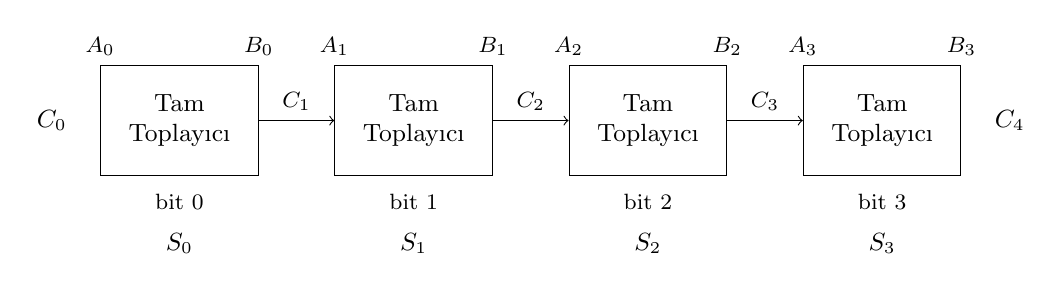
\begin{tikzpicture}[scale=0.85, every node/.style={font=\small},
    fa/.style={draw, minimum width=2cm, minimum height=1.4cm, align=center}]
  % Full adders
  \node[fa] (fa0) at (0, 0) {Tam\\Toplayıcı};
  \node[fa] (fa1) at (3.5, 0) {Tam\\Toplayıcı};
  \node[fa] (fa2) at (7, 0) {Tam\\Toplayıcı};
  \node[fa] (fa3) at (10.5, 0) {Tam\\Toplayıcı};
  % Labels
  \node[below=0.1cm, font=\footnotesize] at (fa0.south) {bit 0};
  \node[below=0.1cm, font=\footnotesize] at (fa1.south) {bit 1};
  \node[below=0.1cm, font=\footnotesize] at (fa2.south) {bit 2};
  \node[below=0.1cm, font=\footnotesize] at (fa3.south) {bit 3};
  % Inputs A, B
  \node[above] at (fa0.north west) {\footnotesize $A_0$};
  \node[above] at (fa0.north east) {\footnotesize $B_0$};
  \node[above] at (fa1.north west) {\footnotesize $A_1$};
  \node[above] at (fa1.north east) {\footnotesize $B_1$};
  \node[above] at (fa2.north west) {\footnotesize $A_2$};
  \node[above] at (fa2.north east) {\footnotesize $B_2$};
  \node[above] at (fa3.north west) {\footnotesize $A_3$};
  \node[above] at (fa3.north east) {\footnotesize $B_3$};
  % Carry chain
  \node[left=0.3cm] at (fa0.west) {$C_0$};
  \draw[->] (fa0.east) -- node[above, font=\footnotesize]{$C_1$} (fa1.west);
  \draw[->] (fa1.east) -- node[above, font=\footnotesize]{$C_2$} (fa2.west);
  \draw[->] (fa2.east) -- node[above, font=\footnotesize]{$C_3$} (fa3.west);
  \node[right=0.3cm] at (fa3.east) {$C_4$};
  % Sum outputs
  \node[below=0.6cm] at (fa0.south) {$S_0$};
  \node[below=0.6cm] at (fa1.south) {$S_1$};
  \node[below=0.6cm] at (fa2.south) {$S_2$};
  \node[below=0.6cm] at (fa3.south) {$S_3$};
\end{tikzpicture}
\caption{4 bitlik dalgalı elde toplayıcı}
\label{fig:dalgali-elde-toplayici}
\end{figure}

Bu yapının dezavantajı, elde sinyalinin en düşük bitten en yüksek bite doğru ``dalga'' halinde yayılmasıdır. $n$ bitlik bir dalgalı elde toplayıcısının toplam gecikmesi $O(n)$ ile orantılıdır çünkü $i$.~basamak, ancak $(i-1)$.~basamağın elde çıkışı kesinleştikten sonra doğru sonucu üretebilir. 64~bitlik bir toplayıcıda bu gecikme kabul edilemez boyutlara ulaşabilir.

Bu sorunu aşmak için geliştirilmiş yöntemler vardır: elde ileriye bakma toplayıcısı (İngilizcesi: \textit{carry lookahead adder}) tüm elde bitlerini eşzamanlı hesaplayarak gecikmeyi $O(\log n)$'ye düşürür. Bu ve diğer hızlı toplayıcı tasarımları Bölüm~\ref{chap:aritmetik}'te ayrıntılı olarak ele alınmaktadır.

\begin{ornek}[B.4]
4 bitlik dalgalı elde toplayıcısı kullanarak $A = 0110$ (6) ile $B = 0101$ (5) sayılarını toplayın. $C_0 = 0$ olarak alın.

\textbf{Çözüm:}

Her basamak sırayla hesaplanır:

\begin{table}[H]
\centering
\begin{tabular}{ccccccc}
\toprule
\textbf{Basamak} & $A_i$ & $B_i$ & $C_i$ & $S_i$ & $C_{i+1}$ \\
\midrule
0 & 0 & 1 & 0 & 1 & 0 \\
1 & 1 & 0 & 0 & 1 & 0 \\
2 & 1 & 1 & 0 & 0 & 1 \\
3 & 0 & 0 & 1 & 1 & 0 \\
\bottomrule
\end{tabular}
\end{table}

Sonuç: $S = 1011$ (11), $C_4 = 0$. Doğrulama: $6 + 5 = 11$. \checkmark
\end{ornek}


% =====================================================
\section{Tasarım Örneği: Tek Vuruşluk Veriyolu Denetim Birimi}

Bölüm~\ref{chap:islemci-tasarimi}'te anlatılan tek vuruşluk veriyolunun denetim birimi, buyrukların gerektirdiği denetim sinyallerini üreten bir birimdir. Bu bölümde bu birimin mantıksal tasarımı yapılmaktadır.

\begin{table}[H]
\centering
\caption{Buyruklar için denetim girişlerinin alacağı değerler}
\label{tab:B.9}
\small
\begin{tabular}{l|cccccccccccc}
\toprule
\textbf{Buyruk} & \rotatebox{90}{\textbf{PS0}} & \rotatebox{90}{\textbf{PS1}} & \rotatebox{90}{\textbf{SnçYzmç}} & \rotatebox{90}{\textbf{YazDen}} & \rotatebox{90}{\textbf{AMBDen}} & \rotatebox{90}{\textbf{BelYaz}} & \rotatebox{90}{\textbf{BelOku}} & \rotatebox{90}{\textbf{SD0}} & \rotatebox{90}{\textbf{SD1}} & \rotatebox{90}{\textbf{GenDen}} & \rotatebox{90}{\textbf{AMB0}} & \rotatebox{90}{\textbf{AMB1}} \\
\midrule
Aritmetik-Mantık & 1 & 0 & 1 & 0 & 0 & 0 & 0 & 0 & 0 & 1 & 1 & 0 \\
Sakla             & 0 & 0 & 0 & 0 & 0 & 1 & 0 & 0 & 0 & 0 & 1 & 0 \\
Yükle             & 0 & 0 & 0 & 0 & 1 & 0 & 1 & 0 & 0 & 0 & 1 & 0 \\
Taşı              & 0 & 0 & 0 & 0 & 0 & 0 & 0 & 0 & 1 & 1 & 0 & 0 \\
Eşitse Dallan     & 0 & 1 & 0 & 1 & 0 & 0 & 0 & 1 & 0 & 0 & 0 & 1 \\
Atla              & 0 & 0 & 0 & 0 & 0 & 0 & 0 & 1 & 0 & 0 & 0 & 0 \\
\bottomrule
\end{tabular}
\end{table}

\begin{table}[H]
\centering
\caption{Denetim birimi girişleri ve çıkışları}
\label{tab:B.10}
\small
\begin{tabular}{cccccc|c|cccccccccccc}
\toprule
$O_5$ & $O_4$ & $O_3$ & $O_2$ & $O_1$ & $O_0$ & $S$ & \rotatebox{90}{\textbf{PS0}} & \rotatebox{90}{\textbf{PS1}} & \rotatebox{90}{\textbf{SnçYzmç}} & \rotatebox{90}{\textbf{YazDen}} & \rotatebox{90}{\textbf{AMBDen}} & \rotatebox{90}{\textbf{BelYaz}} & \rotatebox{90}{\textbf{BelOku}} & \rotatebox{90}{\textbf{SD0}} & \rotatebox{90}{\textbf{SD1}} & \rotatebox{90}{\textbf{GenDen}} & \rotatebox{90}{\textbf{AMB0}} & \rotatebox{90}{\textbf{AMB1}} \\
\midrule
0 & 0 & 0 & 0 & 0 & 0 & 0 & 1 & 0 & 1 & 0 & 0 & 0 & 0 & 0 & 0 & 1 & 1 & 0 \\
0 & 0 & 0 & 0 & 0 & 0 & 1 & 1 & 0 & 1 & 0 & 0 & 0 & 0 & 0 & 0 & 1 & 1 & 0 \\
0 & 0 & 0 & 0 & 0 & 1 & 0 & 0 & 0 & 0 & 0 & 0 & 1 & 0 & 0 & 0 & 0 & 1 & 0 \\
0 & 0 & 0 & 0 & 0 & 1 & 1 & 0 & 0 & 0 & 0 & 0 & 1 & 0 & 0 & 0 & 0 & 1 & 0 \\
0 & 0 & 0 & 0 & 1 & 0 & 0 & 0 & 0 & 0 & 0 & 1 & 0 & 1 & 0 & 0 & 0 & 1 & 0 \\
0 & 0 & 0 & 0 & 1 & 0 & 1 & 0 & 0 & 0 & 0 & 1 & 0 & 1 & 0 & 0 & 0 & 1 & 0 \\
0 & 0 & 0 & 0 & 1 & 1 & 0 & 0 & 0 & 0 & 0 & 0 & 0 & 0 & 0 & 1 & 1 & 0 & 0 \\
0 & 0 & 0 & 0 & 1 & 1 & 1 & 0 & 0 & 0 & 0 & 0 & 0 & 0 & 0 & 1 & 1 & 0 & 0 \\
0 & 0 & 0 & 1 & 0 & 0 & 0 & 0 & 0 & 0 & 0 & 0 & 0 & 0 & 1 & 0 & 0 & 0 & 0 \\
0 & 0 & 0 & 1 & 0 & 0 & 1 & 0 & 1 & 0 & 1 & 0 & 0 & 0 & 1 & 0 & 0 & 0 & 1 \\
0 & 0 & 0 & 1 & 0 & 1 & 0 & 0 & 0 & 0 & 0 & 0 & 0 & 0 & 1 & 0 & 0 & 0 & 0 \\
0 & 0 & 0 & 1 & 0 & 1 & 1 & 0 & 0 & 0 & 0 & 0 & 0 & 0 & 1 & 0 & 0 & 0 & 0 \\
\bottomrule
\end{tabular}
\end{table}

Denetim biriminin tasarımında yalnızca alt 4 bit ($O_2$, $O_1$, $O_0$ ve $S$) kullanılarak sadeleştirme yapılabilir. Aşağıdaki tabloda bu 4 değişkenli doğruluk tablosu verilmiştir:

\begin{table}[H]
\centering
\caption{4 değişkenli denetim birimi doğruluk tablosu}
\label{tab:B.11}
\small
\begin{tabular}{cccc|cccccccccccc}
\toprule
$O_2$ & $O_1$ & $O_0$ & $S$ & \rotatebox{90}{\textbf{PS0}} & \rotatebox{90}{\textbf{PS1}} & \rotatebox{90}{\textbf{SnçYzmç}} & \rotatebox{90}{\textbf{YazDen}} & \rotatebox{90}{\textbf{AMBDen}} & \rotatebox{90}{\textbf{BelYaz}} & \rotatebox{90}{\textbf{BelOku}} & \rotatebox{90}{\textbf{SD0}} & \rotatebox{90}{\textbf{SD1}} & \rotatebox{90}{\textbf{GenDen}} & \rotatebox{90}{\textbf{AMB0}} & \rotatebox{90}{\textbf{AMB1}} \\
\midrule
0 & 0 & 0 & 0 & 1 & 0 & 1 & 0 & 0 & 0 & 0 & 0 & 0 & 1 & 1 & 0 \\
0 & 0 & 0 & 1 & 1 & 0 & 1 & 0 & 0 & 0 & 0 & 0 & 0 & 1 & 1 & 0 \\
0 & 0 & 1 & 0 & 0 & 0 & 0 & 0 & 0 & 1 & 0 & 0 & 0 & 0 & 1 & 0 \\
0 & 0 & 1 & 1 & 0 & 0 & 0 & 0 & 0 & 1 & 0 & 0 & 0 & 0 & 1 & 0 \\
0 & 1 & 0 & 0 & 0 & 0 & 0 & 0 & 1 & 0 & 1 & 0 & 0 & 0 & 1 & 0 \\
0 & 1 & 0 & 1 & 0 & 0 & 0 & 0 & 1 & 0 & 1 & 0 & 0 & 0 & 1 & 0 \\
0 & 1 & 1 & 0 & 0 & 0 & 0 & 0 & 0 & 0 & 0 & 0 & 1 & 1 & 0 & 0 \\
0 & 1 & 1 & 1 & 0 & 0 & 0 & 0 & 0 & 0 & 0 & 0 & 1 & 1 & 0 & 0 \\
1 & 0 & 0 & 0 & 0 & 0 & 0 & 0 & 0 & 0 & 0 & 1 & 0 & 0 & 0 & 0 \\
1 & 0 & 0 & 1 & 0 & 1 & 0 & 1 & 0 & 0 & 0 & 1 & 0 & 0 & 0 & 1 \\
1 & 0 & 1 & 0 & 0 & 0 & 0 & 0 & 0 & 0 & 0 & 1 & 0 & 0 & 0 & 0 \\
1 & 0 & 1 & 1 & 0 & 0 & 0 & 0 & 0 & 0 & 0 & 1 & 0 & 0 & 0 & 0 \\
1 & 1 & 0 & 0 & X & X & X & X & X & X & X & X & X & X & X & X \\
1 & 1 & 0 & 1 & X & X & X & X & X & X & X & X & X & X & X & X \\
1 & 1 & 1 & 0 & X & X & X & X & X & X & X & X & X & X & X & X \\
1 & 1 & 1 & 1 & X & X & X & X & X & X & X & X & X & X & X & X \\
\bottomrule
\end{tabular}
\end{table}

Her denetim çıkışı ayrı bir fonksiyon olarak ele alınır ve Karno haritası ile sadeleştirilir. Şekil~\ref{fig:karno-denetim-1} ve~\ref{fig:karno-denetim-2}'de 12 denetim fonksiyonunun Karno haritaları toplu olarak verilmiştir:

% --- TikZ makrosu: Karno haritası (denetim bölümü, 4 değişken) ---
\newcommand{\denetimkarno}[5]{%%
\begin{tikzpicture}[scale=0.55]
    \draw (0,0) grid (4,4);
    \node[above] at (0.5, 4) {\tiny 00};
    \node[above] at (1.5, 4) {\tiny 01};
    \node[above] at (2.5, 4) {\tiny 11};
    \node[above] at (3.5, 4) {\tiny 10};
    \node[left] at (0, 3.5) {\tiny 00};
    \node[left] at (0, 2.5) {\tiny 01};
    \node[left] at (0, 1.5) {\tiny 11};
    \node[left] at (0, 0.5) {\tiny 10};
    #1 #2 #3 #4 #5
\end{tikzpicture}%%
}

\begin{figure}[H]
\centering
% --- Satır 1: PS0, PS1, SnçYzmç ---
\subcaptionbox{PS0\label{fig:B.12}}{%%
\denetimkarno%%
  {\node at (0.5,3.5) {1}; \node at (1.5,3.5) {1}; \node at (2.5,3.5) {0}; \node at (3.5,3.5) {0};}%%
  {\node at (0.5,2.5) {0}; \node at (1.5,2.5) {0}; \node at (2.5,2.5) {0}; \node at (3.5,2.5) {0};}%%
  {\node at (0.5,1.5) {X}; \node at (1.5,1.5) {X}; \node at (2.5,1.5) {X}; \node at (3.5,1.5) {X};}%%
  {\node at (0.5,0.5) {0}; \node at (1.5,0.5) {0}; \node at (2.5,0.5) {1}; \node at (3.5,0.5) {1};}%%
  {\draw[rounded corners=3pt, thick, sinyalkirmizi, opacity=0.6] (-0.05,3.05) rectangle (1.95,3.95);}%%
}\hfill
\subcaptionbox{PS1\label{fig:B.13}}{%%
\denetimkarno%%
  {\node at (0.5,3.5) {0}; \node at (1.5,3.5) {0}; \node at (2.5,3.5) {0}; \node at (3.5,3.5) {0};}%%
  {\node at (0.5,2.5) {0}; \node at (1.5,2.5) {0}; \node at (2.5,2.5) {0}; \node at (3.5,2.5) {0};}%%
  {\node at (0.5,1.5) {X}; \node at (1.5,1.5) {X}; \node at (2.5,1.5) {X}; \node at (3.5,1.5) {X};}%%
  {\node at (0.5,0.5) {0}; \node at (1.5,0.5) {1}; \node at (2.5,0.5) {0}; \node at (3.5,0.5) {0};}%%
  {\draw[rounded corners=3pt, thick, sinyalkirmizi, opacity=0.6] (1.05,0.05) rectangle (1.95,0.95);}%%
}\hfill
\subcaptionbox{SnçYzmç\label{fig:B.14}}{%%
\denetimkarno%%
  {\node at (0.5,3.5) {1}; \node at (1.5,3.5) {1}; \node at (2.5,3.5) {0}; \node at (3.5,3.5) {0};}%%
  {\node at (0.5,2.5) {0}; \node at (1.5,2.5) {0}; \node at (2.5,2.5) {0}; \node at (3.5,2.5) {0};}%%
  {\node at (0.5,1.5) {X}; \node at (1.5,1.5) {X}; \node at (2.5,1.5) {X}; \node at (3.5,1.5) {X};}%%
  {\node at (0.5,0.5) {0}; \node at (1.5,0.5) {0}; \node at (2.5,0.5) {0}; \node at (3.5,0.5) {0};}%%
  {\draw[rounded corners=3pt, thick, sinyalkirmizi, opacity=0.6] (-0.05,3.05) rectangle (1.95,3.95);}%%
}

\bigskip
% --- Satır 2: YazDen, AMBDen, BelYaz ---
\subcaptionbox{YazDen\label{fig:B.15}}{%%
\denetimkarno%%
  {\node at (0.5,3.5) {0}; \node at (1.5,3.5) {0}; \node at (2.5,3.5) {0}; \node at (3.5,3.5) {0};}%%
  {\node at (0.5,2.5) {0}; \node at (1.5,2.5) {0}; \node at (2.5,2.5) {0}; \node at (3.5,2.5) {0};}%%
  {\node at (0.5,1.5) {X}; \node at (1.5,1.5) {X}; \node at (2.5,1.5) {X}; \node at (3.5,1.5) {X};}%%
  {\node at (0.5,0.5) {0}; \node at (1.5,0.5) {1}; \node at (2.5,0.5) {0}; \node at (3.5,0.5) {0};}%%
  {\draw[rounded corners=3pt, thick, sinyalkirmizi, opacity=0.6] (1.05,0.05) rectangle (1.95,0.95);}%%
}\hfill
\subcaptionbox{AMBDen\label{fig:B.16}}{%%
\denetimkarno%%
  {\node at (0.5,3.5) {0}; \node at (1.5,3.5) {0}; \node at (2.5,3.5) {0}; \node at (3.5,3.5) {0};}%%
  {\node at (0.5,2.5) {1}; \node at (1.5,2.5) {1}; \node at (2.5,2.5) {0}; \node at (3.5,2.5) {0};}%%
  {\node at (0.5,1.5) {X}; \node at (1.5,1.5) {X}; \node at (2.5,1.5) {X}; \node at (3.5,1.5) {X};}%%
  {\node at (0.5,0.5) {0}; \node at (1.5,0.5) {0}; \node at (2.5,0.5) {0}; \node at (3.5,0.5) {0};}%%
  {\draw[rounded corners=3pt, thick, sinyalkirmizi, opacity=0.6] (-0.05,2.05) rectangle (1.95,2.95);}%%
}\hfill
\subcaptionbox{BelYaz\label{fig:B.17}}{%%
\denetimkarno%%
  {\node at (0.5,3.5) {0}; \node at (1.5,3.5) {0}; \node at (2.5,3.5) {1}; \node at (3.5,3.5) {1};}%%
  {\node at (0.5,2.5) {0}; \node at (1.5,2.5) {0}; \node at (2.5,2.5) {0}; \node at (3.5,2.5) {0};}%%
  {\node at (0.5,1.5) {X}; \node at (1.5,1.5) {X}; \node at (2.5,1.5) {X}; \node at (3.5,1.5) {X};}%%
  {\node at (0.5,0.5) {0}; \node at (1.5,0.5) {0}; \node at (2.5,0.5) {0}; \node at (3.5,0.5) {0};}%%
  {\draw[rounded corners=3pt, thick, sinyalkirmizi, opacity=0.6] (2.05,3.05) rectangle (3.95,3.95);}%%
}
\caption{Denetim fonksiyonları Karno haritaları -- 1.\ grup}
\label{fig:karno-denetim-1}
\end{figure}

\begin{figure}[H]
\centering
% --- Satır 1: BelOku, SD0, SD1 ---
\subcaptionbox{BelOku\label{fig:B.18}}{%%
\denetimkarno%%
  {\node at (0.5,3.5) {0}; \node at (1.5,3.5) {0}; \node at (2.5,3.5) {0}; \node at (3.5,3.5) {0};}%%
  {\node at (0.5,2.5) {1}; \node at (1.5,2.5) {1}; \node at (2.5,2.5) {0}; \node at (3.5,2.5) {0};}%%
  {\node at (0.5,1.5) {X}; \node at (1.5,1.5) {X}; \node at (2.5,1.5) {X}; \node at (3.5,1.5) {X};}%%
  {\node at (0.5,0.5) {0}; \node at (1.5,0.5) {0}; \node at (2.5,0.5) {0}; \node at (3.5,0.5) {0};}%%
  {\draw[rounded corners=3pt, thick, sinyalkirmizi, opacity=0.6] (-0.05,2.05) rectangle (1.95,2.95);}%%
}\hfill
\subcaptionbox{SD0\label{fig:B.19}}{%%
\denetimkarno%%
  {\node at (0.5,3.5) {0}; \node at (1.5,3.5) {0}; \node at (2.5,3.5) {0}; \node at (3.5,3.5) {0};}%%
  {\node at (0.5,2.5) {0}; \node at (1.5,2.5) {0}; \node at (2.5,2.5) {0}; \node at (3.5,2.5) {0};}%%
  {\node at (0.5,1.5) {X}; \node at (1.5,1.5) {X}; \node at (2.5,1.5) {X}; \node at (3.5,1.5) {X};}%%
  {\node at (0.5,0.5) {1}; \node at (1.5,0.5) {1}; \node at (2.5,0.5) {1}; \node at (3.5,0.5) {1};}%%
  {\draw[rounded corners=3pt, thick, sinyalkirmizi, opacity=0.6] (-0.05,0.05) rectangle (3.95,0.95);}%%
}\hfill
\subcaptionbox{SD1\label{fig:B.20}}{%%
\denetimkarno%%
  {\node at (0.5,3.5) {0}; \node at (1.5,3.5) {0}; \node at (2.5,3.5) {0}; \node at (3.5,3.5) {0};}%%
  {\node at (0.5,2.5) {0}; \node at (1.5,2.5) {0}; \node at (2.5,2.5) {1}; \node at (3.5,2.5) {1};}%%
  {\node at (0.5,1.5) {X}; \node at (1.5,1.5) {X}; \node at (2.5,1.5) {X}; \node at (3.5,1.5) {X};}%%
  {\node at (0.5,0.5) {0}; \node at (1.5,0.5) {0}; \node at (2.5,0.5) {0}; \node at (3.5,0.5) {0};}%%
  {\draw[rounded corners=3pt, thick, sinyalkirmizi, opacity=0.6] (2.05,2.05) rectangle (3.95,2.95);}%%
}

\bigskip
% --- Satır 2: GenDen, AMB0, AMB1 ---
\subcaptionbox{GenDen\label{fig:B.21}}{%%
\denetimkarno%%
  {\node at (0.5,3.5) {1}; \node at (1.5,3.5) {1}; \node at (2.5,3.5) {0}; \node at (3.5,3.5) {0};}%%
  {\node at (0.5,2.5) {0}; \node at (1.5,2.5) {0}; \node at (2.5,2.5) {1}; \node at (3.5,2.5) {1};}%%
  {\node at (0.5,1.5) {X}; \node at (1.5,1.5) {X}; \node at (2.5,1.5) {X}; \node at (3.5,1.5) {X};}%%
  {\node at (0.5,0.5) {0}; \node at (1.5,0.5) {0}; \node at (2.5,0.5) {0}; \node at (3.5,0.5) {0};}%%
  {\draw[rounded corners=3pt, thick, sinyalkirmizi, opacity=0.6] (-0.05,3.05) rectangle (1.95,3.95); \draw[rounded corners=3pt, thick, sinyalmavi, opacity=0.6] (2.05,2.05) rectangle (3.95,2.95);}%%
}\hfill
\subcaptionbox{AMB0\label{fig:B.22}}{%%
\denetimkarno%%
  {\node at (0.5,3.5) {1}; \node at (1.5,3.5) {1}; \node at (2.5,3.5) {1}; \node at (3.5,3.5) {1};}%%
  {\node at (0.5,2.5) {1}; \node at (1.5,2.5) {1}; \node at (2.5,2.5) {0}; \node at (3.5,2.5) {0};}%%
  {\node at (0.5,1.5) {X}; \node at (1.5,1.5) {X}; \node at (2.5,1.5) {X}; \node at (3.5,1.5) {X};}%%
  {\node at (0.5,0.5) {0}; \node at (1.5,0.5) {0}; \node at (2.5,0.5) {0}; \node at (3.5,0.5) {0};}%%
  {\draw[rounded corners=3pt, thick, sinyalkirmizi, opacity=0.6] (-0.05,3.05) rectangle (3.95,3.95); \draw[rounded corners=3pt, thick, sinyalmavi, opacity=0.6] (-0.05,2.05) rectangle (1.95,3.95);}%%
}\hfill
\subcaptionbox{AMB1\label{fig:B.23}}{%%
\denetimkarno%%
  {\node at (0.5,3.5) {0}; \node at (1.5,3.5) {0}; \node at (2.5,3.5) {0}; \node at (3.5,3.5) {0};}%%
  {\node at (0.5,2.5) {0}; \node at (1.5,2.5) {0}; \node at (2.5,2.5) {0}; \node at (3.5,2.5) {0};}%%
  {\node at (0.5,1.5) {X}; \node at (1.5,1.5) {X}; \node at (2.5,1.5) {X}; \node at (3.5,1.5) {X};}%%
  {\node at (0.5,0.5) {0}; \node at (1.5,0.5) {1}; \node at (2.5,0.5) {0}; \node at (3.5,0.5) {0};}%%
  {\draw[rounded corners=3pt, thick, sinyalkirmizi, opacity=0.6] (1.05,0.05) rectangle (1.95,0.95);}%%
}
\caption{Denetim fonksiyonları Karno haritaları -- 2.\ grup}
\label{fig:karno-denetim-2}
\end{figure}


\section{Flip-Floplar}

Flip-floplar ikilik düzende bir değer tutulabilen, mantık kapılarından oluşmuş yapılardır. Ardışıl devrelerin temel yapı taşlarıdır ve bir bit bilgi saklayabilirler. Dört temel flip-flop türü bulunmaktadır: RS, D, T ve JK.


\subsection{RS Flip-flop}

RS (\emph{Reset-Set}) flip-flopu, çapraz bağlanmış iki VEYA DEĞİL kapısından oluşur. İki girişi (S ve R) ve iki çıkışı ($Q$ ve $\overline{Q}$) vardır. S (Set) girişi flip-flopu 1 durumuna, R (Reset) girişi ise 0 durumuna getirir.

\begin{figure}[H]
\centering
\begin{tikzpicture}[kapiboy, scale=0.8, transform shape]
  % İki çapraz bağlı NOR kapısı
  \node[nor gate US, draw, thick, fill=blokgri] (nor1) at (3, 1.5) {};
  \node[nor gate US, draw, thick, fill=blokgri] (nor2) at (3, -1.5) {};

  % S girişi
  \draw (nor1.input 1) -- ++(-1.5,0) node[left] {\footnotesize $S$};
  % R girişi
  \draw (nor2.input 2) -- ++(-1.5,0) node[left] {\footnotesize $R$};

  % Çapraz bağlantılar
  \draw (nor1.output) -- ++(0.5,0) coordinate (q1out);
  \draw (nor2.output) -- ++(0.5,0) coordinate (q2out);

  \draw (q1out) -- ++(0.3,0) |- ++(0.2,-0.5) coordinate (fb1);
  \draw (fb1) -- ++(-0,-1.1) -| (nor2.input 1);

  \draw (q2out) -- ++(0.3,0) |- ++(0.2,0.5) coordinate (fb2);
  \draw (fb2) -- ++(-0,1.1) -| (nor1.input 2);

  % Çıkışlar
  \draw (q1out) -- ++(1.8,0) node[right] {\footnotesize $Q$};
  \draw (q2out) -- ++(1.8,0) node[right] {\footnotesize $\overline{Q}$};
\end{tikzpicture}
\caption{RS Flip-flop}
\label{fig:B.24}
\end{figure}

\begin{table}[H]
\centering
\caption{RS Flip-flop doğruluk tablosu}
\label{tab:B.12}
\begin{tabular}{cc|cc|l}
\toprule
$S$ & $R$ & $Q$ & $\overline{Q}$ & \textbf{Açıklama} \\
\midrule
0 & 0 & $Q(t)$ & $\overline{Q(t)}$ & Değişme yok \\
0 & 1 & 0 & 1 & Sıfırla \\
1 & 0 & 1 & 0 & Kur \\
1 & 1 & -- & -- & Kararsız durum \\
\bottomrule
\end{tabular}
\end{table}

RS flip-flopun çalışma prensibi şu şekildedir: $S = 0$ ve $R = 0$ olduğunda flip-flop mevcut durumunu korur. $S = 1$ ve $R = 0$ olduğunda çıkış $Q = 1$ olur (kur). $S = 0$ ve $R = 1$ olduğunda çıkış $Q = 0$ olur (sıfırla). $S = 1$ ve $R = 1$ durumu ise kararsız durumdur ve kaçınılması gereken bir durumdur; çünkü her iki çıkış da aynı anda 0 olur ve bu durum flip-flopun doğru çalışmasını engeller.

RS flip-flop, VEYA DEĞİL kapıları yerine VE DEĞİL kapıları ile de oluşturulabilir. VE DEĞİL kapıları ile yapılan RS flip-flopunda girişler aktif-düşük olarak çalışır.


\subsection{D Flip-flop}

D (\emph{Data}) flip-flopu, tek bir veri girişi ($D$) ve bir saat girişi olan flip-flop türüdür. Saat sinyalinin etkin kenarında (yükselen veya düşen kenar) $D$ girişindeki değer $Q$ çıkışına aktarılır. D flip-flopu 1 bitlik veri saklamak için kullanılır ve yazmaçların temel yapı taşıdır.

\begin{figure}[H]
\centering
\begin{tikzpicture}[scale=1]
  % Flip-flop kutusu
  \node[flipflop, minimum width=2.2cm, minimum height=2.8cm] (ff) at (0,0) {};
  \node[font=\footnotesize\bfseries] at (0, 1.0) {D FF};

  % D girişi
  \draw (ff.west |- 0,0.4) -- ++(-1.2,0) node[left] {\footnotesize $D$};
  \node[ffgiris, right] at ([xshift=2pt]ff.west |- 0,0.4) {$D$};

  % Saat girişi (üçgen sembolü ile)
  \draw (ff.west |- 0,-0.4) -- ++(-1.2,0) node[left] {\footnotesize CLK};
  \draw ([xshift=2pt]ff.west |- 0,-0.55) -- ++(0.2,0.15) -- ++(-0.2,0.15);

  % Q çıkışı
  \draw (ff.east |- 0,0.4) -- ++(1.2,0) node[right] {\footnotesize $Q$};
  \node[ffcikis, left] at ([xshift=-2pt]ff.east |- 0,0.4) {$Q$};

  % Q̅ çıkışı
  \draw (ff.east |- 0,-0.4) -- ++(1.2,0) node[right] {\footnotesize $\overline{Q}$};
  \node[ffcikis, left] at ([xshift=-2pt]ff.east |- 0,-0.4) {$\overline{Q}$};
\end{tikzpicture}
\caption{D Flip-flop}
\label{fig:B.25}
\end{figure}

\begin{table}[H]
\centering
\caption{D Flip-flop doğruluk tablosu}
\label{tab:B.13}
\begin{tabular}{cc|c}
\toprule
$Q(t)$ & $D$ & $Q(t+1)$ \\
\midrule
0 & 0 & 0 \\
0 & 1 & 1 \\
1 & 0 & 0 \\
1 & 1 & 1 \\
\bottomrule
\end{tabular}
\end{table}


\subsection{T Flip-flop}

T (\emph{Toggle}) flip-flopu, tek bir girişi ($T$) olan flip-flop türüdür. $T = 1$ olduğunda flip-flopun durumu tersine döner (toggle), $T = 0$ olduğunda mevcut durum korunur. T flip-flopu özellikle sayaç devrelerinde yaygın olarak kullanılır.

\begin{figure}[H]
\centering
\begin{tikzpicture}[scale=1]
  % Flip-flop kutusu
  \node[flipflop, minimum width=2.2cm, minimum height=2.8cm] (ff) at (0,0) {};
  \node[font=\footnotesize\bfseries] at (0, 1.0) {T FF};

  % T girişi
  \draw (ff.west |- 0,0.4) -- ++(-1.2,0) node[left] {\footnotesize $T$};
  \node[ffgiris, right] at ([xshift=2pt]ff.west |- 0,0.4) {$T$};

  % Saat girişi
  \draw (ff.west |- 0,-0.4) -- ++(-1.2,0) node[left] {\footnotesize CLK};
  \draw ([xshift=2pt]ff.west |- 0,-0.55) -- ++(0.2,0.15) -- ++(-0.2,0.15);

  % Q çıkışı
  \draw (ff.east |- 0,0.4) -- ++(1.2,0) node[right] {\footnotesize $Q$};
  \node[ffcikis, left] at ([xshift=-2pt]ff.east |- 0,0.4) {$Q$};

  % Q̅ çıkışı
  \draw (ff.east |- 0,-0.4) -- ++(1.2,0) node[right] {\footnotesize $\overline{Q}$};
  \node[ffcikis, left] at ([xshift=-2pt]ff.east |- 0,-0.4) {$\overline{Q}$};
\end{tikzpicture}
\caption{T Flip-flop}
\label{fig:B.26}
\end{figure}

\begin{table}[H]
\centering
\caption{T Flip-flop doğruluk tablosu}
\label{tab:B.14}
\begin{tabular}{cc|c}
\toprule
$T$ & $Q(t)$ & $Q(t+1)$ \\
\midrule
0 & 0 & 0 \\
0 & 1 & 1 \\
1 & 0 & 1 \\
1 & 1 & 0 \\
\bottomrule
\end{tabular}
\end{table}


\subsection{JK Flip-flop}

JK flip-flopu, RS flip-flopun geliştirilmiş halidir. İki girişi ($J$ ve $K$) vardır. RS flip-floptaki kararsız durum ($S = R = 1$) problemi JK flip-flopunda çözülmüştür. $J = K = 1$ olduğunda flip-flopun durumu tersine döner.

\begin{figure}[H]
\centering
\begin{tikzpicture}[scale=1]
  % Flip-flop kutusu
  \node[flipflop, minimum width=2.2cm, minimum height=3.2cm] (ff) at (0,0) {};
  \node[font=\footnotesize\bfseries] at (0, 1.2) {JK FF};

  % J girişi
  \draw (ff.west |- 0,0.6) -- ++(-1.2,0) node[left] {\footnotesize $J$};
  \node[ffgiris, right] at ([xshift=2pt]ff.west |- 0,0.6) {$J$};

  % K girişi
  \draw (ff.west |- 0,-0.6) -- ++(-1.2,0) node[left] {\footnotesize $K$};
  \node[ffgiris, right] at ([xshift=2pt]ff.west |- 0,-0.6) {$K$};

  % Saat girişi
  \draw (ff.west |- 0,0) -- ++(-1.2,0) node[left] {\footnotesize CLK};
  \draw ([xshift=2pt]ff.west |- 0,-0.15) -- ++(0.2,0.15) -- ++(-0.2,0.15);

  % Q çıkışı
  \draw (ff.east |- 0,0.5) -- ++(1.2,0) node[right] {\footnotesize $Q$};
  \node[ffcikis, left] at ([xshift=-2pt]ff.east |- 0,0.5) {$Q$};

  % Q̅ çıkışı
  \draw (ff.east |- 0,-0.5) -- ++(1.2,0) node[right] {\footnotesize $\overline{Q}$};
  \node[ffcikis, left] at ([xshift=-2pt]ff.east |- 0,-0.5) {$\overline{Q}$};
\end{tikzpicture}
\caption{JK Flip-flop}
\label{fig:B.27}
\end{figure}

\begin{table}[H]
\centering
\caption{JK Flip-flop doğruluk tablosu}
\label{tab:B.15}
\begin{tabular}{cc|c|l}
\toprule
$J$ & $K$ & $Q(t+1)$ & \textbf{Açıklama} \\
\midrule
0 & 0 & $Q(t)$ & Değişme yok \\
0 & 1 & 0 & Sıfırla \\
1 & 0 & 1 & Kur \\
1 & 1 & $\overline{Q(t)}$ & Tersle \\
\bottomrule
\end{tabular}
\end{table}

JK flip-flopun çalışma prensibi şu şekildedir: $J = 0$ ve $K = 0$ olduğunda flip-flop mevcut durumunu korur. $J = 0$ ve $K = 1$ olduğunda çıkış $Q = 0$ olur (sıfırla). $J = 1$ ve $K = 0$ olduğunda çıkış $Q = 1$ olur (kur). $J = 1$ ve $K = 1$ olduğunda ise çıkış tersine döner ve $Q(t+1) = \overline{Q(t)}$ olur. Bu özellik JK flip-flopu RS flip-flopundan ayıran en önemli farktır.


% =====================================================
\section{Yazmaçlar}
\label{sec:ekB-yazmaclar}
\index{yazmaç}

Yazmaç (İngilizcesi: \textit{register}), birden fazla flip-flopun bir araya getirilmesiyle oluşturulan ve birden çok bitlik bir veriyi eşzamanlı olarak saklayabilen birimdir. Bir $n$ bitlik yazmaç, $n$ adet D flip-flopundan oluşur ve her biri ortak bir saat sinyaliyle tetiklenir.

\subsection{Koşut Yüklemeli Yazmaç}
\index{koşut yüklemeli yazmaç}

En basit yazmaç türü olan \textbf{koşut yüklemeli yazmaç}ta tüm bitler aynı anda (tek bir saat vuruşunda) yüklenir. Her D flip-flopunun girişine ilgili veri biti bağlanır; saat sinyalinin yükselen kenarında tüm bitler eşzamanlı olarak güncellenir.

\begin{figure}[H]
\centering
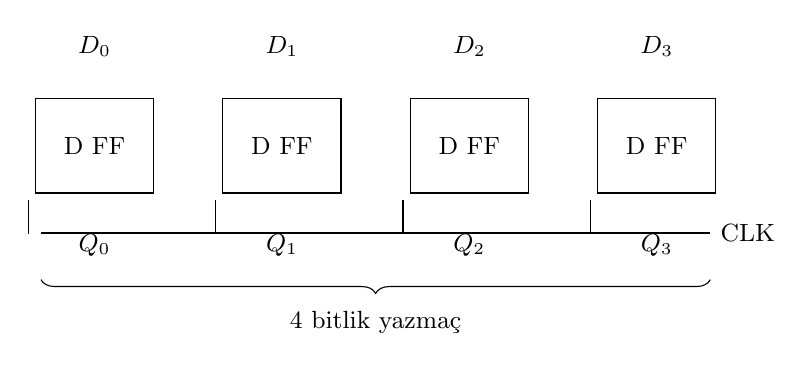
\begin{tikzpicture}[scale=0.85, every node/.style={font=\small},
    dff/.style={draw, minimum width=1.5cm, minimum height=1.2cm}]
  \foreach \i in {0,1,2,3} {
    \node[dff] (d\i) at (2.8*\i, 0) {D FF};
    \node[above=0.4cm] at (d\i.north) {$D_\i$};
    \node[below=0.4cm] at (d\i.south) {$Q_\i$};
  }
  % Clock line
  \draw[thick] (-0.8, -1.3) -- (9.2, -1.3) node[right] {CLK};
  \foreach \i in {0,1,2,3} {
    \draw (d\i.south west) ++(-0.1,-0.1) -- ++(0,-0.5);
  }
  % Brace for label
  \draw[decorate, decoration={brace, amplitude=5pt, mirror}] (-0.8, -2) -- (9.2, -2) node[midway, below=8pt] {4 bitlik yazmaç};
\end{tikzpicture}
\caption{4 bitlik koşut yüklemeli yazmaç}
\label{fig:kosut-yazmac}
\end{figure}

Uygulamada yazmaçlara genellikle bir ``yükleme etkinleştirme'' (İngilizcesi: \textit{load enable}) denetim sinyali eklenir. Bu sinyal aktif olmadığında yazmaç, saat vuruşlarına karşın mevcut değerini korur; aktif olduğunda ise yeni veri yüklenir. Bu sayede yazmaç yalnızca istenildiğinde güncellenir.

\subsection{Kaydırma Yazmacı}
\index{kaydırma yazmacı}

Kaydırma yazmacı (İngilizcesi: \textit{shift register}), her saat vuruşunda saklanan bit dizisini bir konum sağa ya da sola kaydıran bir yazmaçtır. Her D flip-flopunun çıkışı ($Q$), bir sonraki (sağa kaydırmada) ya da bir önceki (sola kaydırmada) flip-flopun girişine ($D$) bağlanır.

Kaydırma yazmaçları çarpma (sola kaydırma $= \times 2$) ve bölme (sağa kaydırma $= \div 2$) işlemlerinde, seri-koşut veri dönüştürmede ve iletişim arabirimlerinde yaygın olarak kullanılır.

\begin{ornek}[B.5]
4 bitlik bir kaydırma yazmacında başlangıç değeri $1011$ olsun. Sağa üç kez kaydırma yapıldığında ve boşalan en soldaki bite 0 yazıldığında sırayla hangi değerler elde edilir?

\textbf{Çözüm:}

\begin{table}[H]
\centering
\begin{tabular}{cl}
\toprule
\textbf{Saat vuruşu} & \textbf{Yazmaç içeriği} \\
\midrule
Başlangıç & $1011$ \\
1.~vuruş   & $0101$ \\
2.~vuruş   & $0010$ \\
3.~vuruş   & $0001$ \\
\bottomrule
\end{tabular}
\end{table}

Başlangıç değeri $1011_2 = 11_{10}$ idi. Her sağa kaydırma ikiye bölmeye karşılık gelir: $11 \to 5 \to 2 \to 1$ (kesirli kısımlar atılır).
\end{ornek}


% =====================================================
\section{Sayaçlar}
\label{sec:sayaclar}
\index{sayaç}

Sayaç (İngilizcesi: \textit{counter}), her saat vuruşunda değerini belirli bir düzende artıran ya da azaltan ardışıl devredir. Sayaçlar, işlemcilerde program sayacı (İngilizcesi: \textit{program counter}) olarak, zamanlama devrelerinde, bellek adresleme birimlerinde ve olay sayma işlemlerinde kullanılır.

\subsection{Eşzamanlı İkili Sayaç}
\index{eşzamanlı sayaç}

Eşzamanlı (İngilizcesi: \textit{synchronous}) sayaçta tüm flip-floplar aynı saat sinyaliyle tetiklenir. $n$ bitlik bir yukarı sayaç, $0$'dan $2^n - 1$'e kadar sayar ve sonra sıfıra döner. Sayacı gerçekleştirmek için T flip-flopları kullanılır: en düşük bit ($T_0$) her zaman terslenirken, $i$.~bit ancak kendisinden düşük tüm bitler $1$ olduğunda terslenmelidir.

\[
T_0 = 1, \qquad T_1 = Q_0, \qquad T_2 = Q_0 \cdot Q_1, \qquad T_i = \prod_{j=0}^{i-1} Q_j
\]

\begin{ornek}[B.6]
3 bitlik eşzamanlı yukarı sayacın sayma dizisini yazın.

\textbf{Çözüm:}

\begin{table}[H]
\centering
\begin{tabular}{c|ccc}
\toprule
\textbf{Saat} & $Q_2$ & $Q_1$ & $Q_0$ \\
\midrule
0 & 0 & 0 & 0 \\
1 & 0 & 0 & 1 \\
2 & 0 & 1 & 0 \\
3 & 0 & 1 & 1 \\
4 & 1 & 0 & 0 \\
5 & 1 & 0 & 1 \\
6 & 1 & 1 & 0 \\
7 & 1 & 1 & 1 \\
(8 & 0 & 0 & 0) \\
\bottomrule
\end{tabular}
\end{table}

Sayaç $0$'dan $7$'ye kadar sayar ve saat vuruşu 8'de sıfıra döner. $T_0 = 1$ olduğu için en düşük bit her vuruşta değişir. $T_1 = Q_0$ olduğu için $Q_1$, yalnızca $Q_0 = 1$ olduğu vuruşlarda değişir. $T_2 = Q_0 \cdot Q_1$ olduğu için $Q_2$, ancak her iki alt bit de $1$ olduğunda değişir.
\end{ornek}

\subsection{Eşzamansız (Dalgalı) Sayaç}
\index{eşzamansız sayaç}

Eşzamansız (İngilizcesi: \textit{asynchronous} veya \textit{ripple}) sayaçta yalnızca ilk flip-flop doğrudan saat sinyaliyle tetiklenir; sonraki her flip-flopun saat girişi, bir önceki flip-flopun çıkışına bağlanır. Bu yapı daha basittir ancak elde sinyalinin ``dalga'' halinde yayılmasına benzer şekilde, terslenme sinyali basamaktan basamağa gecikmeyle ilerler. Bu nedenle yüksek hızlı uygulamalarda eşzamanlı sayaçlar tercih edilir.


% =====================================================
\section{Durum Tablosu ile Tasarım Örneği}

Durum makineleri, ardışıl devrelerin tasarımında kullanılan temel bir yöntemdir. Bir durum makinesinin davranışı, mevcut durumu ve girişlerine göre belirlenir. Her saat çevriminde durum makinesi bir sonraki duruma geçer ve buna uygun çıkışlar üretir.

\begin{figure}[H]
\centering
\begin{tikzpicture}[node distance=3.5cm]
  % Durumlar
  \node[durum, minimum size=1.6cm] (bos) {Boş};
  \node[durum, minimum size=1.6cm, right of=bos] (dol) {Dolduruluyor};
  \node[durum, minimum size=1.6cm, right of=dol] (full) {Dolu};

  % Geçişler
  \draw[durumok] (bos) to node[above, font=\footnotesize] {Başlat} (dol);
  \draw[durumok] (dol) to node[above, font=\footnotesize] {Doldu} (full);
  \draw[durumok, bend left=30] (full) to node[below, font=\footnotesize] {Boşalt} (bos);

  % Döngüler
  \draw[durumdongu] (bos) to node[above, font=\footnotesize] {Bekle} (bos);
  \draw[durumdongu] (dol) to node[above, font=\footnotesize] {Doldur} (dol);
  \draw[->, >=Stealth, thick, loop above, looseness=8] (full) to node[above, font=\footnotesize] {Bekle} (full);
\end{tikzpicture}
\caption{Havuz dolum örneği durum şeması}
\label{fig:B.28}
\end{figure}

Bu bölümde daha karmaşık bir örnek olan bir yarışma sistemi tasarlanacaktır. Yarışmada iki yarışmacı (A ve B) bulunmaktadır ve son iki sorunun cevapları değerlendirilmektedir. Sistemin çıkışları aşağıdaki tabloda gösterilmiştir:

\begin{table}[H]
\centering
\caption{A ve B'nin doğru sayılarına göre çıktı tablosu}
\label{tab:B.16}
\begin{tabular}{l|c}
\toprule
\textbf{Durum} & \textbf{Çıkış} \\
\midrule
Eşit & 000 \\
A, B'den 2 fazla doğru & 001 \\
A, B'den 1 fazla doğru & 010 \\
B, A'dan 1 fazla doğru & 011 \\
B, A'dan 2 fazla doğru & 100 \\
\bottomrule
\end{tabular}
\end{table}

Sistem üç durumda bulunabilir:
\begin{itemize}
    \item Eşit durumu: $xy = 00$
    \item A önde durumu: $xy = 01$
    \item B önde durumu: $xy = 10$
\end{itemize}

\begin{figure}[H]
\centering
\begin{tikzpicture}[node distance=4cm]
  % Durumlar
  \node[durum, minimum size=1.8cm, align=center] (esit) {Eşit\\\scriptsize $xy{=}00$};
  \node[durum, minimum size=1.8cm, align=center, below right of=esit, xshift=1cm] (bonde) {B Önde\\\scriptsize $xy{=}10$};
  \node[durum, minimum size=1.8cm, align=center, below left of=esit, xshift=-1cm] (aonde) {A Önde\\\scriptsize $xy{=}01$};

  % Geçişler
  % Eşit -> A Önde (A doğru, B yanlış)
  \draw[durumok, bend left=20] (esit) to node[left, font=\footnotesize] {$AB{=}10$} (aonde);
  % A Önde -> Eşit (B doğru)
  \draw[durumok, bend left=20] (aonde) to node[right, font=\footnotesize] {$AB{=}01$} (esit);
  % Eşit -> B Önde (B doğru, A yanlış)
  \draw[durumok, bend left=20] (esit) to node[right, font=\footnotesize] {$AB{=}01$} (bonde);
  % B Önde -> Eşit (A doğru)
  \draw[durumok, bend left=20] (bonde) to node[left, font=\footnotesize] {$AB{=}10$} (esit);

  % Döngüler
  \draw[->, >=Stealth, thick, loop above, looseness=8] (esit) to node[above, font=\footnotesize] {$AB{=}00,11$} (esit);
  \draw[->, >=Stealth, thick, loop left, looseness=8] (aonde) to node[left, font=\footnotesize] {$AB{=}10$} (aonde);
  \draw[->, >=Stealth, thick, loop right, looseness=8] (bonde) to node[right, font=\footnotesize] {$AB{=}01$} (bonde);

  % Ek geçişler (A Önde -> aynı durumda kalma / diğer geçişler)
  \draw[durumok, bend left=20] (aonde) to node[below, font=\footnotesize] {$AB{=}00$} (esit.-170);
  \draw[durumok, bend left=20] (bonde) to node[below, font=\footnotesize] {$AB{=}00$} (esit.-10);
\end{tikzpicture}
\caption{Yarışma örneği durum şeması}
\label{fig:B.29}
\end{figure}

\begin{table}[H]
\centering
\caption{Yarışma örneği durumlara göre çıkış değerleri}
\label{tab:B.17}
\small
\begin{tabular}{cccc|cc|ccc}
\toprule
$x$ & $y$ & $A$ & $B$ & $x(t+1)$ & $y(t+1)$ & $\text{Ç}_2$ & $\text{Ç}_1$ & $\text{Ç}_0$ \\
\midrule
0 & 0 & 0 & 0 & 0 & 0 & 0 & 0 & 0 \\
0 & 0 & 0 & 1 & 1 & 0 & 0 & 1 & 1 \\
0 & 0 & 1 & 0 & 0 & 1 & 0 & 1 & 0 \\
0 & 0 & 1 & 1 & 0 & 0 & 0 & 0 & 0 \\
0 & 1 & 0 & 0 & 0 & 0 & 0 & 1 & 0 \\
0 & 1 & 0 & 1 & 0 & 0 & 0 & 0 & 0 \\
0 & 1 & 1 & 0 & 0 & 1 & 0 & 0 & 1 \\
0 & 1 & 1 & 1 & 0 & 1 & 0 & 1 & 0 \\
1 & 0 & 0 & 0 & 0 & 0 & 0 & 1 & 1 \\
1 & 0 & 0 & 1 & 1 & 0 & 1 & 0 & 0 \\
1 & 0 & 1 & 0 & 0 & 0 & 0 & 0 & 0 \\
1 & 0 & 1 & 1 & 1 & 0 & 0 & 1 & 1 \\
1 & 1 & X & X & X & X & X & X & X \\
\bottomrule
\end{tabular}
\end{table}

Tasarımda JK flip-flopları kullanılacaktır. JK flip-flopunun geçiş tablosu aşağıda verilmiştir:

\begin{table}[H]
\centering
\caption{JK flip-flopta $J$ ve $K$ değerleri için doğruluk tablosu}
\label{tab:B.18}
\begin{tabular}{cc|cc|l}
\toprule
$x$ & $x(t+1)$ & $J_x$ & $K_x$ & \textbf{Açıklama} \\
\midrule
0 & 0 & 0 & X & Sıfırla ya da aynı kal \\
0 & 1 & 1 & X & Birle ya da tersle \\
1 & 0 & X & 1 & Sıfırla ya da tersle \\
1 & 1 & X & 0 & Birle ya da aynı kal \\
\bottomrule
\end{tabular}
\end{table}

Bu geçiş tablosu kullanılarak tüm sistemin doğruluk tablosu oluşturulur:

\begin{table}[H]
\centering
\caption{Tüm sistem için doğruluk tablosu}
\label{tab:B.19}
\small
\begin{tabular}{cccc|cc|ccc|cccc}
\toprule
$x$ & $y$ & $A$ & $B$ & $x(t+1)$ & $y(t+1)$ & $\text{Ç}_2$ & $\text{Ç}_1$ & $\text{Ç}_0$ & $J_x$ & $K_x$ & $J_y$ & $K_y$ \\
\midrule
0 & 0 & 0 & 0 & 0 & 0 & 0 & 0 & 0 & 0 & X & 0 & X \\
0 & 0 & 0 & 1 & 1 & 0 & 0 & 1 & 1 & 1 & X & 0 & X \\
0 & 0 & 1 & 0 & 0 & 1 & 0 & 1 & 0 & 0 & X & 1 & X \\
0 & 0 & 1 & 1 & 0 & 0 & 0 & 0 & 0 & 0 & X & 0 & X \\
0 & 1 & 0 & 0 & 0 & 0 & 0 & 1 & 0 & 0 & X & X & 1 \\
0 & 1 & 0 & 1 & 0 & 0 & 0 & 0 & 0 & 0 & X & X & 1 \\
0 & 1 & 1 & 0 & 0 & 1 & 0 & 0 & 1 & 0 & X & X & 0 \\
0 & 1 & 1 & 1 & 0 & 1 & 0 & 1 & 0 & 0 & X & X & 0 \\
1 & 0 & 0 & 0 & 0 & 0 & 0 & 1 & 1 & X & 1 & 0 & X \\
1 & 0 & 0 & 1 & 1 & 0 & 1 & 0 & 0 & X & 0 & 0 & X \\
1 & 0 & 1 & 0 & 0 & 0 & 0 & 0 & 0 & X & 1 & 0 & X \\
1 & 0 & 1 & 1 & 1 & 0 & 0 & 1 & 1 & X & 0 & 0 & X \\
1 & 1 & 0 & 0 & X & X & X & X & X & X & X & X & X \\
1 & 1 & 0 & 1 & X & X & X & X & X & X & X & X & X \\
1 & 1 & 1 & 0 & X & X & X & X & X & X & X & X & X \\
1 & 1 & 1 & 1 & X & X & X & X & X & X & X & X & X \\
\bottomrule
\end{tabular}
\end{table}

Her bir çıkış fonksiyonu ve flip-flop girişleri Karno haritası ile sadeleştirilir:

\begin{figure}[H]
\centering
\begin{tikzpicture}[scale=0.8]
    \draw (0,0) grid (4,4);
    \node[above] at (0.5, 4) {\footnotesize 00};
    \node[above] at (1.5, 4) {\footnotesize 01};
    \node[above] at (2.5, 4) {\footnotesize 11};
    \node[above] at (3.5, 4) {\footnotesize 10};
    \node[left] at (0, 3.5) {\footnotesize 00};
    \node[left] at (0, 2.5) {\footnotesize 01};
    \node[left] at (0, 1.5) {\footnotesize 11};
    \node[left] at (0, 0.5) {\footnotesize 10};
    \node[above left] at (0, 4) {\footnotesize $xy$\textbackslash $AB$};
    % Row 00: 0,0,0,0
    \node at (0.5,3.5) {0}; \node at (1.5,3.5) {0}; \node at (2.5,3.5) {0}; \node at (3.5,3.5) {0};
    % Row 01: 0,0,0,0
    \node at (0.5,2.5) {0}; \node at (1.5,2.5) {0}; \node at (2.5,2.5) {0}; \node at (3.5,2.5) {0};
    % Row 11: X,X,X,X
    \node at (0.5,1.5) {X}; \node at (1.5,1.5) {X}; \node at (2.5,1.5) {X}; \node at (3.5,1.5) {X};
    % Row 10: 0,1,0,0
    \node at (0.5,0.5) {0}; \node at (1.5,0.5) {1}; \node at (2.5,0.5) {0}; \node at (3.5,0.5) {0};
    \draw[rounded corners=3pt, thick, sinyalkirmizi, opacity=0.6] (1.05,0.05) rectangle (1.95,0.95);
\end{tikzpicture}
\caption{$\text{Ç}_2$ çıkışı Karno haritası}
\label{fig:B.30}
\end{figure}

\begin{figure}[H]
\centering
\begin{tikzpicture}[scale=0.8]
    \draw (0,0) grid (4,4);
    \node[above] at (0.5, 4) {\footnotesize 00};
    \node[above] at (1.5, 4) {\footnotesize 01};
    \node[above] at (2.5, 4) {\footnotesize 11};
    \node[above] at (3.5, 4) {\footnotesize 10};
    \node[left] at (0, 3.5) {\footnotesize 00};
    \node[left] at (0, 2.5) {\footnotesize 01};
    \node[left] at (0, 1.5) {\footnotesize 11};
    \node[left] at (0, 0.5) {\footnotesize 10};
    \node[above left] at (0, 4) {\footnotesize $xy$\textbackslash $AB$};
    % Row 00: 0,1,0,1
    \node at (0.5,3.5) {0}; \node at (1.5,3.5) {1}; \node at (2.5,3.5) {0}; \node at (3.5,3.5) {1};
    % Row 01: 1,0,1,0
    \node at (0.5,2.5) {1}; \node at (1.5,2.5) {0}; \node at (2.5,2.5) {1}; \node at (3.5,2.5) {0};
    % Row 11: X,X,X,X
    \node at (0.5,1.5) {X}; \node at (1.5,1.5) {X}; \node at (2.5,1.5) {X}; \node at (3.5,1.5) {X};
    % Row 10: 1,0,1,0
    \node at (0.5,0.5) {1}; \node at (1.5,0.5) {0}; \node at (2.5,0.5) {1}; \node at (3.5,0.5) {0};
    % Dama tahtası deseni: XOR fonksiyonu (Karno gruplandırması uygulanamaz)
    % 1 olan hücreler daire ile işaretlenir
    \foreach \x/\y in {1.5/3.5, 3.5/3.5, 0.5/2.5, 2.5/2.5, 0.5/0.5, 2.5/0.5} {
        \draw[thick, sinyalkirmizi, opacity=0.6] (\x,\y) circle (0.4);
    }
    % X hücreleri de dahil edilebilir
    \foreach \x/\y in {0.5/1.5, 1.5/1.5, 2.5/1.5, 3.5/1.5} {
        \draw[thick, sinyalmavi, opacity=0.4] (\x,\y) circle (0.4);
    }
\end{tikzpicture}
\caption{$\text{Ç}_1$ çıkışı Karno haritası}
\label{fig:B.31}
\end{figure}

\begin{figure}[H]
\centering
\begin{tikzpicture}[scale=0.8]
    \draw (0,0) grid (4,4);
    \node[above] at (0.5, 4) {\footnotesize 00};
    \node[above] at (1.5, 4) {\footnotesize 01};
    \node[above] at (2.5, 4) {\footnotesize 11};
    \node[above] at (3.5, 4) {\footnotesize 10};
    \node[left] at (0, 3.5) {\footnotesize 00};
    \node[left] at (0, 2.5) {\footnotesize 01};
    \node[left] at (0, 1.5) {\footnotesize 11};
    \node[left] at (0, 0.5) {\footnotesize 10};
    \node[above left] at (0, 4) {\footnotesize $xy$\textbackslash $AB$};
    % Row 00: 0,1,0,0
    \node at (0.5,3.5) {0}; \node at (1.5,3.5) {1}; \node at (2.5,3.5) {0}; \node at (3.5,3.5) {0};
    % Row 01: 0,0,0,1
    \node at (0.5,2.5) {0}; \node at (1.5,2.5) {0}; \node at (2.5,2.5) {0}; \node at (3.5,2.5) {1};
    % Row 11: X,X,X,X
    \node at (0.5,1.5) {X}; \node at (1.5,1.5) {X}; \node at (2.5,1.5) {X}; \node at (3.5,1.5) {X};
    % Row 10: 1,0,1,0
    \node at (0.5,0.5) {1}; \node at (1.5,0.5) {0}; \node at (2.5,0.5) {1}; \node at (3.5,0.5) {0};
    \draw[rounded corners=3pt, thick, sinyalkirmizi, opacity=0.6] (1.05,3.05) rectangle (1.95,3.95);
    \draw[rounded corners=3pt, thick, sinyalmavi, opacity=0.6] (3.05,2.05) rectangle (3.95,2.95);
    \draw[rounded corners=3pt, thick, sinyalyesil, opacity=0.6] (-0.05,0.05) rectangle (0.95,0.95);
    \draw[rounded corners=3pt, thick, orange, opacity=0.6] (2.05,0.05) rectangle (2.95,0.95);
\end{tikzpicture}
\caption{$\text{Ç}_0$ çıkışı Karno haritası}
\label{fig:B.32}
\end{figure}

\begin{figure}[H]
\centering
\begin{tikzpicture}[scale=0.8]
    \draw (0,0) grid (4,4);
    \node[above] at (0.5, 4) {\footnotesize 00};
    \node[above] at (1.5, 4) {\footnotesize 01};
    \node[above] at (2.5, 4) {\footnotesize 11};
    \node[above] at (3.5, 4) {\footnotesize 10};
    \node[left] at (0, 3.5) {\footnotesize 00};
    \node[left] at (0, 2.5) {\footnotesize 01};
    \node[left] at (0, 1.5) {\footnotesize 11};
    \node[left] at (0, 0.5) {\footnotesize 10};
    \node[above left] at (0, 4) {\footnotesize $xy$\textbackslash $AB$};
    % Row 00: 0,1,0,0
    \node at (0.5,3.5) {0}; \node at (1.5,3.5) {1}; \node at (2.5,3.5) {0}; \node at (3.5,3.5) {0};
    % Row 01: 0,0,0,0
    \node at (0.5,2.5) {0}; \node at (1.5,2.5) {0}; \node at (2.5,2.5) {0}; \node at (3.5,2.5) {0};
    % Row 11: X,X,X,X
    \node at (0.5,1.5) {X}; \node at (1.5,1.5) {X}; \node at (2.5,1.5) {X}; \node at (3.5,1.5) {X};
    % Row 10: X,X,X,X
    \node at (0.5,0.5) {X}; \node at (1.5,0.5) {X}; \node at (2.5,0.5) {X}; \node at (3.5,0.5) {X};
    \draw[rounded corners=3pt, thick, sinyalkirmizi, opacity=0.6] (1.05,3.05) rectangle (1.95,3.95);
\end{tikzpicture}
\caption{$J_x$ fonksiyonu Karno haritası}
\label{fig:B.33}
\end{figure}

\begin{figure}[H]
\centering
\begin{tikzpicture}[scale=0.8]
    \draw (0,0) grid (4,4);
    \node[above] at (0.5, 4) {\footnotesize 00};
    \node[above] at (1.5, 4) {\footnotesize 01};
    \node[above] at (2.5, 4) {\footnotesize 11};
    \node[above] at (3.5, 4) {\footnotesize 10};
    \node[left] at (0, 3.5) {\footnotesize 00};
    \node[left] at (0, 2.5) {\footnotesize 01};
    \node[left] at (0, 1.5) {\footnotesize 11};
    \node[left] at (0, 0.5) {\footnotesize 10};
    \node[above left] at (0, 4) {\footnotesize $xy$\textbackslash $AB$};
    % Row 00: X,X,X,X
    \node at (0.5,3.5) {X}; \node at (1.5,3.5) {X}; \node at (2.5,3.5) {X}; \node at (3.5,3.5) {X};
    % Row 01: X,X,X,X
    \node at (0.5,2.5) {X}; \node at (1.5,2.5) {X}; \node at (2.5,2.5) {X}; \node at (3.5,2.5) {X};
    % Row 11: X,X,X,X
    \node at (0.5,1.5) {X}; \node at (1.5,1.5) {X}; \node at (2.5,1.5) {X}; \node at (3.5,1.5) {X};
    % Row 10: 1,0,0,1
    \node at (0.5,0.5) {1}; \node at (1.5,0.5) {0}; \node at (2.5,0.5) {0}; \node at (3.5,0.5) {1};
    \draw[rounded corners=3pt, thick, sinyalkirmizi, opacity=0.6] (-0.05,0.05) rectangle (0.95,0.95);
    \draw[rounded corners=3pt, thick, sinyalmavi, opacity=0.6] (3.05,0.05) rectangle (3.95,0.95);
\end{tikzpicture}
\caption{$K_x$ fonksiyonu Karno haritası}
\label{fig:B.34}
\end{figure}

\begin{figure}[H]
\centering
\begin{tikzpicture}[scale=0.8]
    \draw (0,0) grid (4,4);
    \node[above] at (0.5, 4) {\footnotesize 00};
    \node[above] at (1.5, 4) {\footnotesize 01};
    \node[above] at (2.5, 4) {\footnotesize 11};
    \node[above] at (3.5, 4) {\footnotesize 10};
    \node[left] at (0, 3.5) {\footnotesize 00};
    \node[left] at (0, 2.5) {\footnotesize 01};
    \node[left] at (0, 1.5) {\footnotesize 11};
    \node[left] at (0, 0.5) {\footnotesize 10};
    \node[above left] at (0, 4) {\footnotesize $xy$\textbackslash $AB$};
    % Row 00: 0,0,0,1
    \node at (0.5,3.5) {0}; \node at (1.5,3.5) {0}; \node at (2.5,3.5) {0}; \node at (3.5,3.5) {1};
    % Row 01: X,X,X,X
    \node at (0.5,2.5) {X}; \node at (1.5,2.5) {X}; \node at (2.5,2.5) {X}; \node at (3.5,2.5) {X};
    % Row 11: X,X,X,X
    \node at (0.5,1.5) {X}; \node at (1.5,1.5) {X}; \node at (2.5,1.5) {X}; \node at (3.5,1.5) {X};
    % Row 10: 0,0,0,0
    \node at (0.5,0.5) {0}; \node at (1.5,0.5) {0}; \node at (2.5,0.5) {0}; \node at (3.5,0.5) {0};
    \draw[rounded corners=3pt, thick, sinyalkirmizi, opacity=0.6] (3.05,3.05) rectangle (3.95,3.95);
\end{tikzpicture}
\caption{$J_y$ fonksiyonu Karno haritası}
\label{fig:B.35}
\end{figure}

\begin{figure}[H]
\centering
\begin{tikzpicture}[scale=0.8]
    \draw (0,0) grid (4,4);
    \node[above] at (0.5, 4) {\footnotesize 00};
    \node[above] at (1.5, 4) {\footnotesize 01};
    \node[above] at (2.5, 4) {\footnotesize 11};
    \node[above] at (3.5, 4) {\footnotesize 10};
    \node[left] at (0, 3.5) {\footnotesize 00};
    \node[left] at (0, 2.5) {\footnotesize 01};
    \node[left] at (0, 1.5) {\footnotesize 11};
    \node[left] at (0, 0.5) {\footnotesize 10};
    \node[above left] at (0, 4) {\footnotesize $xy$\textbackslash $AB$};
    % Row 00: X,X,X,X
    \node at (0.5,3.5) {X}; \node at (1.5,3.5) {X}; \node at (2.5,3.5) {X}; \node at (3.5,3.5) {X};
    % Row 01: 1,1,0,0
    \node at (0.5,2.5) {1}; \node at (1.5,2.5) {1}; \node at (2.5,2.5) {0}; \node at (3.5,2.5) {0};
    % Row 11: X,X,X,X
    \node at (0.5,1.5) {X}; \node at (1.5,1.5) {X}; \node at (2.5,1.5) {X}; \node at (3.5,1.5) {X};
    % Row 10: X,X,X,X
    \node at (0.5,0.5) {X}; \node at (1.5,0.5) {X}; \node at (2.5,0.5) {X}; \node at (3.5,0.5) {X};
    \draw[rounded corners=3pt, thick, sinyalkirmizi, opacity=0.6] (-0.05,2.05) rectangle (1.95,2.95);
\end{tikzpicture}
\caption{$K_y$ fonksiyonu Karno haritası}
\label{fig:B.36}
\end{figure}

Sistemin son hali için mantık kapılarıyla ve gereken giriş çıkışların birbirine bağlanmasıyla elde edilecek devreye A ve B yarışmacılarının soruları doğru ya da yanlış cevaplama bilgileri girilerek sonuç elde edilir.


\section{Özet}

Bu ekte, sayısal devrelerin temelini oluşturan kavramlar ve yapı taşları ele alınmıştır.

\begin{center}
\small
\begin{tabular}{lp{10cm}}
\toprule
\textbf{Kavram} & \textbf{Özet} \\
\midrule
Mantık Kapıları & VE, VEYA, DEĞİL, TÜVE, TÜVEYA ve XOR kapıları dijital devrelerin temel yapı taşlarıdır. Her kapının davranışı doğruluk tablosuyla tanımlanır. \\
Boole Cebri & Mantık fonksiyonlarının cebirsel gösterimi ve sadeleştirilmesi için kullanılır. Mini terimler ve maksi terimler, herhangi bir fonksiyonun standart biçimde ifadesini sağlar. \\
Karno Haritası & Boole fonksiyonlarının görsel olarak sadeleştirilmesini sağlayan bir yöntemdir; 2, 3 ve 4 değişkenli fonksiyonlarda etkilidir. \\
Kod Çözücü ve Çoklayıcı & Kod çözücü $n$ bitlik girişi $2^n$ çıkıştan birine yönlendirir. Çoklayıcı ise $2^n$ girişten birini seçerek tek çıkışa aktarır. \\
Toplayıcılar & Yarım toplayıcı, tam toplayıcı ve dalgalı elde toplayıcı, ikilik toplama işlemini donanım düzeyinde gerçekleştirir. \\
Flip-Floplar & RS, D, T ve JK flip-flopları, tek bitlik bilgi depolayan ardışıl devre elemanlarıdır. Saat sinyaliyle tetiklenirler. \\
Yazmaçlar & Birden fazla flip-flopun bir araya gelmesiyle oluşan çok bitlik depolama birimleridir. Koşut yüklemeli ve kaydırma yazmaçları yaygın türleridir. \\
Sayaçlar & Her saat vuruşunda değerini artıran ya da azaltan ardışıl devrelerdir. Eşzamanlı ve eşzamansız türleri vardır. \\
Durum Makineleri & Ardışıl devrelerin tasarımında kullanılır. Mevcut durum ve girişlere göre bir sonraki durum ve çıkışlar belirlenir. \\
\bottomrule
\end{tabular}
\end{center}


\section*{Alıştırmalar}
\addcontentsline{toc}{section}{Alıştırmalar}
\label{sec:ekB-alistirmalar}

\begin{alistirma}[\kolay]
Aşağıdaki ikilik sayıların 2'ye tümleyenini bulun:
\begin{enumerate}[(a)]
    \item $(101010)_2$
    \item $(110011)_2$
    \item $(10000000)_2$
\end{enumerate}
\end{alistirma}

\begin{alistirma}[\kolay]
VE, VEYA ve DEĞİL kapılarının doğruluk tablolarını yazın. TÜVE kapısının, bir VE kapısı ve ardından gelen bir DEĞİL kapısıyla eşdeğer olduğunu doğruluk tablosuyla gösterin.
\end{alistirma}

\begin{alistirma}[\orta]
Üç girişli ($x$, $y$, $z$) bir fonksiyon, girişlerin çoğunluğu 1 olduğunda 1 çıkışı veren bir çoğunluk devresini temsil etmektedir. Bu fonksiyonun doğruluk tablosunu oluşturun ve Boole ifadesini yazın.
\end{alistirma}

\begin{alistirma}[\orta]
Aşağıdaki Boole fonksiyonlarını Karno haritası kullanarak sadeleştirin:
\begin{enumerate}[(a)]
    \item $F(x,y,z) = \Sigma(0, 2, 4, 5, 6)$
    \item $F(w,x,y,z) = \Sigma(0, 1, 2, 4, 5, 6, 8, 9, 12, 13, 14)$
\end{enumerate}
\end{alistirma}

\begin{alistirma}[\orta]
4 girişli ve 16 çıkışlı bir kod çözücü tasarlayın. Doğruluk tablosunu oluşturun.
\end{alistirma}

\begin{alistirma}[\orta]
Bir yarım toplayıcının doğruluk tablosunu oluşturun ve $S$ (toplam) ile $C$ (elde) çıkışları için Boole denklemlerini yazın. Devre şemasını çizin.
\end{alistirma}

\begin{alistirma}[\orta]
Bir tam toplayıcının iki yarım toplayıcı ve bir VEYA kapısı kullanılarak nasıl gerçekleştirileceğini gösterin. Bağlantı şemasını çizin ve doğruluk tablosuyla doğrulayın.
\end{alistirma}

\begin{alistirma}[\orta]
4 bitlik dalgalı elde toplayıcısı kullanarak $A = 1001$ ile $B = 0111$ sayılarını toplayın. Her basamaktaki $A_i$, $B_i$, $C_i$, $S_i$ ve $C_{i+1}$ değerlerini tablo halinde gösterin. Sonucu hem ikilik hem de onluk tabanda doğrulayın.
\end{alistirma}

\begin{alistirma}[\orta]
JK flip-flop kullanarak bir T flip-flopu nasıl elde edebilirsiniz? Bağlantı şemasını çizin ve doğruluk tablosuyla doğrulayın.
\end{alistirma}

\begin{alistirma}[\orta]
4 bitlik bir kaydırma yazmacında başlangıç değeri $1100$ olsun. Sola dört kez kaydırma yapıldığında (boşalan en sağdaki bite 0 yazılarak) sırayla hangi değerler elde edilir? Her adımdaki onluk tabandaki karşılığı nedir?
\end{alistirma}

\begin{alistirma}[\zor]
Üç bitlik bir eşzamanlı yukarı sayıcıyı T flip-flopları kullanarak tasarlayın. Durum tablosunu, her bir flip-flopun $T$ giriş denklemini ve devre şemasını çizin.
\end{alistirma}

\begin{alistirma}[\zor]
8:1 çoklayıcı kullanarak $F(A, B, C) = \Sigma(1, 2, 6, 7)$ fonksiyonunu gerçekleştirin. Bağlantı şemasını çizin.
\end{alistirma}

\begin{alistirma}[\zor]
Dalgalı elde toplayıcısının en kötü durum gecikmesi neden $O(n)$ ile orantılıdır? 32 bitlik bir toplayıcıda her tam toplayıcının elde gecikmesi 2~ns ise en kötü durum toplam gecikmesini hesaplayın. Bu gecikme 1~GHz'lik bir saat sıklığı için kabul edilebilir midir?
\end{alistirma}

\begin{alistirma}[\zor]
Bir trafik ışığı denetleyicisi tasarlayın. İki yönlü bir kavşakta Kuzey--Güney (KG) ve Doğu--Batı (DB) yönleri için kırmızı, sarı ve yeşil ışıkları denetleyen bir durum makinesi oluşturun. Geçerli durumları, geçişleri ve her durumdaki çıkışları belirleyerek durum diyagramını çizin.
\end{alistirma}
